%  LaTeX report template by Lloren Fanals Batllori

%%%%%%%%%%%%%%%%%%%%%%%%%%%%%%%%%%%%%%%%%%%
% DOCUMENT LAYOUT AND GEOMETRY
%%%%%%%%%%%%%%%%%%%%%%%%%%%%%%%%%%%%%%%%%%%

% Set document default font size, dimensions and geometry
\documentclass[11pt, a4paper, x11names]{report}
\usepackage[a4paper, left=30mm, right=20mm, top=25mm, bottom=25mm]{geometry}
\setlength{\headsep}{20pt}
\setlength{\footskip}{25pt}
\sloppy % Force a new line when surpassing the right margin

% Set accepted characters
\usepackage[utf8]{inputenc} % Use UTF-8 characters

% Set document header and footer
\usepackage{fancyhdr}
\fancypagestyle{plain}{
	\fancyhf{}
	\fancyhead[L]{\footnotesize{\LaTeX \ template}}
	\fancyhead[R]{\footnotesize{Llorenç Fanals Batllori}}
	\fancyfoot[R]{\footnotesize{\thepage}}
}
\pagestyle{plain} % Make header and footer appear the same in every page

%%%%%%%%%%%%%%%%%%%%%%%%%%%%%%%%%%%%%%%%%%%
% MODIFICATIONS FROM DEFAULT: figures, tables, equations, bibliography
%%%%%%%%%%%%%%%%%%%%%%%%%%%%%%%%%%%%%%%%%%%

% Rename default LaTeX structures
\renewcommand{\contentsname}{Table of contents}
\renewcommand{\chaptername}{Chapter}
\renewcommand{\listfigurename}{Figures list}
\renewcommand{\listtablename}{Tables list}
\renewcommand{\appendixname}{Appendix}

% Tables and figures captions
\usepackage{caption}
% Figures
\captionsetup[figure]{labelsep=period}
\renewcommand{\thefigure}{Figure \arabic{figure}}
\captionsetup[figure]{font=footnotesize, skip=11pt}
% Tables
\captionsetup[table]{labelsep=period}
\renewcommand{\thetable}{Table \arabic{table}}
\captionsetup[table]{font=footnotesize, skip=11pt}

\setlength{\belowcaptionskip}{-20pt}

% Images
\usepackage{graphicx}
\graphicspath{{images/}} % default image directory
\usepackage{float}

% Count figures, tables and equations as 1, 2, 3.. for all the document
\usepackage{chngcntr}
\counterwithout{figure}{chapter}
\counterwithout{table}{chapter}
\counterwithout{equation}{chapter}
% Split equations and other stuff
\usepackage{mathtools}

% Links and reference colors
\usepackage[svgnames]{xcolor}
\usepackage{color}
\usepackage[colorlinks]{hyperref} % href, links

\usepackage{hyperref} 
\hypersetup{
	colorlinks=true,
	linkcolor=, 
	filecolor=magenta,
	urlcolor=cyan,
}


%%%%%%%%%%%%%%%%%%%%%%%%%%%%%%%%%%%%%%%%%%%
% ELECTRONICS SCHEMATICS 
%%%%%%%%%%%%%%%%%%%%%%%%%%%%%%%%%%%%%%%%%%%

\usepackage[american]{circuitikz} % american/european
\usepackage{siunitx} % \SI units, useful for equations too
\usetikzlibrary{calc} % relative positions


%%%%%%%%%%%%%%%%%%%%%%%%%%%%%%%%%%%%%%%%%%%
% SPACINGS
%%%%%%%%%%%%%%%%%%%%%%%%%%%%%%%%%%%%%%%%%%%

\usepackage{parskip}
\setlength{\parindent}{0pt}

\usepackage{titlesec}
\linespread{1.3} % Separation between paragraph lines
\setlength{\parskip}{20pt plus 2pt minus 2pt} % Spacing between paragraphs
% \titlespacing{command}{left spacing}{before spacing}{after spacing}[right]
% Chapter
\titlespacing*{\chapter}{0pt}{-38pt}{-11pt}
\titleformat{\chapter}[hang] % Keep writing after the chapter number
{\normalfont\fontsize{16}{16}\bfseries}{\thechapter.}{0.4em}{\bfseries}
% Section
\titlespacing*{\section}{0pt}{11pt}{11pt}
\titleformat{\section}[hang] % Keep writing after the chapter number
{\normalfont\fontsize{11}{16}\bfseries}{\thesection.}{0.4em}{\bfseries}
% Section
\titlespacing*{\subsection}{0pt}{11pt}{11pt}
\titleformat{\subsection}[hang] % Keep writing after the chapter number
{\normalfont\fontsize{11}{16}\bfseries}{\thesubsection.}{0.4em}{\bfseries}

% Equation separations with the rest of the elements
\makeatletter
\g@addto@macro{\normalsize}{%
	\setlength{\abovedisplayskip}{6pt}
	\setlength{\abovedisplayshortskip}{6pt}
	\setlength{\belowdisplayskip}{6pt}
	\setlength{\belowdisplayshortskip}{6pt}
}
\makeatother

% Use tables that offer spaces
\usepackage{tabu} % tabularx


%%%%%%%%%%%%%%%%%%%%%%%%%%%%%%%%%%%%%%%%%%%
% PLOTS
%%%%%%%%%%%%%%%%%%%%%%%%%%%%%%%%%%%%%%%%%%%

\usepackage{tikz}
\usepackage{pgfplots}
\pgfplotsset{compat=1.17}
\usetikzlibrary{fit}
\usetikzlibrary{arrows}
\usepackage{tikz-3dplot}

% % Save figures as PDFs, avoid recomputing them every time
% \usetikzlibrary{external}
% \tikzexternalize[prefix=cache/]
 

%%%%%%%%%%%%%%%%%%%%%%%%%%%%%%%%%%%%%%%%%%%
% CUSTOM COMMANDS
%%%%%%%%%%%%%%%%%%%%%%%%%%%%%%%%%%%%%%%%%%%

\newcommand{\infigure}[4]{
	\begin{figure} [h]
		\centering
		\includegraphics[scale=#1]{./images/#2}
		\caption{#3}
		\label{#4}
	\end{figure}
}

% Input Inkscape SVG figures, Giles Castel
\usepackage{import}
\usepackage{xifthen}
\usepackage{pdfpages}
\usepackage{transparent}

\newcommand{\ink}[4]{
	\begin{figure}
		\centering
		\def\svgscale{#1}
		\import{./images/}{#2.pdf_tex}
		\caption{#3}
		\label{#4}
	\end{figure}
	\normalsize
}


%%%%%%%%%%%%%%%%%%%%%%%%%%%%%%%%%%%%%%%%%%%
% Statement environment
%%%%%%%%%%%%%%%%%%%%%%%%%%%%%%%%%%%%%%%%%%%

% https://tex.stackexchange.com/questions/451343/alternative-box-style-table-and-curve
\usepackage{amsmath,amssymb}
\usepackage{lmodern}
\usepackage[most]{tcolorbox}
\usepackage{cleveref} % cref{label} to get the section that contains the exercise

% Exercise box, contains a title
\makeatletter
\tcbset{
    exbox/.style 2 args={%
		parbox=false,
        enhanced,
        breakable,
        colback=black!15!white,
        colframe=black,
        attach boxed title to top left={yshift*=-\tcboxedtitleheight},
		title={\textbf{#2}},
        boxed title size=title,
        boxed title style={%
            sharp corners,
            rounded corners=northwest,
            colback=tcbcolframe,
            boxrule=0pt,
        },
        underlay boxed title={%
            \path[fill=tcbcolframe] (title.south west)--(title.south east)
                to[out=0, in=180] ([xshift=5mm]title.east)--
                (title.center-|frame.east)
                [rounded corners=\kvtcb@arc] |-
                (frame.north) -| cycle;
        },
		before skip=20pt plus 2pt, after skip=20pt plus 2pt,
        #1
    },
}
\makeatother

\newtcolorbox{exbox}[3][]{%
    exbox={#1}{#2},
	label={#3}
}

% Partial exercise box, doesn't contain a title
\makeatletter
\tcbset{
    pexbox/.style ={%
		parbox=false,
        enhanced,
        breakable,
        colback=black!4!white,
        colframe=black,
		before skip=20pt plus 2pt, after skip=20pt plus 2pt,
        #1
    },
}
\makeatother

\newtcolorbox{pexbox}[2][]{%
	pexbox={#1},
	label={#2}
}


%%%%%%%%%%%%%%%%%%%%%%%%%%%%%%%%%%%%%%%%%%%
% CODE
%%%%%%%%%%%%%%%%%%%%%%%%%%%%%%%%%%%%%%%%%%%

% Code listings
\usepackage{listings}
\lstset{aboveskip=22pt,belowskip=0pt} % lstlisting box separation with surrounding text

% VHDL
\lstdefinelanguage{VHDL}{
	morekeywords=[1]{
		library, use, all, entity, is, port, in, out, end, architecture, of, begin, and, or, not, downto, all, if, elsif, when, then, case, process, event, else, generic, signal, not, variable, others, out, integer, range, to, generate, xor, for, STD_LOGIC_VECTOR, STD_LOGIC, IEEE, STD_LOGIC_1164, NUMERIC_STD, STD_LOGIC_ARTIH, STD_LOGIC_UNSIGNED, std_logic_vector, std_logic},
	morecomment=[l]-
}
\colorlet{keyword}{blue!100!black!80}
\colorlet{comment}{green!80!black!90}
\lstdefinestyle{vhdl}{
	language	= VHDL,
	basicstyle  = \linespread{1.1} \scriptsize \ttfamily,
	keywordstyle = [1]\color{keyword}\bfseries,
	keywordstyle = [2]\color{keyword}\bfseries,
	commentstyle = \color{comment},
	breaklines = true,
	tabsize = 4,
	numbers = left,
	numberstyle = {\tiny \color{black}},
	numbersep = 9pt,
	frame = single,
	literate={á}{{\'a}}1 {é}{{\'e}}1 {ó}{{\'o}}1 {í}{{\'i}}1 {ú}{{\'u}}1  {à}{\`{a}}1 {è}{\`{e}}1  {ò}{\`{o}}    1  {ï}{\"\i}1  {ç}{\c{c}}1 , % To type Llorenç and other catalan/spanish words
}

% C
\lstdefinestyle{C}{ %use this for awesome C code
	language	= C,
	basicstyle  = \linespread{1.1} \scriptsize \ttfamily,
	showstringspaces	= false,
	keywordstyle	= \bfseries\color{red!80!black},
	commentstyle	= \color{green!40!black},
	identifierstyle	= \color{black},
	stringstyle	= \color{orange},
	breaklines	= true,
	% postbreak=\llap{\scriptsize\textcolor{blue}{$\hookrightarrow$}\kern0.25em}
	tabsize = 4,
	numbers = left,
	numberstyle = {\tiny \color{black}},
	numbersep = 9pt,
	frame = single,
	literate={á}{{\'a}}1 {é}{{\'e}}1 {ó}{{\'o}}1 {í}{{\'i}}1 {ú}{{\'u}}1  {à}{\`{a}}1 {è}{\`{e}}1  {ò}{\`{o}}    1  {ï}{\"\i}1  {ç}{\c{c}}1 , % To type Llorenç and other catalan/spanish words
	literate={{**}}{{{**}\allowbreak}}1, % To break * lines, not the most elegant solution
}


%%%%%%%%%%%%%%%%%%%%%%%%%%%%%%%%%%%%%%%%%%%
% MISCELLANEOUS 
%%%%%%%%%%%%%%%%%%%%%%%%%%%%%%%%%%%%%%%%%%%

\usepackage[UKenglish]{datetime}
\synctex=1 % Forward and backward interaction with the .pdf

%%%%%%%%%%%%%%%%%%%%%%%%%%%%%%%%%%%%%%%%%%%
%%%%%%%%%%%%%%%%%%%%%%%%%%%%%%%%%%%%%%%%%%%
%%%%%%%%%%%%%%%%%%%%%%%%%%%%%%%%%%%%%%%%%%%

\begin{document}

% Titlepage
\begin{titlepage}
	\begin{center}
		\vspace*{1cm} % the skip at the begginning of the page is not discarded
		
		\huge

	\hrule
		\textbf{Deliver 01} % Deliver number
		\vspace{0.5cm}

		\Large
		\textbf{This is the report title}

		\vspace{0.5cm}
	\hrule
		
		\vspace{2.5cm}
		\Large

		\textbf{Llorenç Fanals Batllori}

		\vspace{-0.4cm}
		\texttt{\href{mailto:llorenc.fanals@estudiantat.upc.edu}{\color{black}{llorenc.fanals@estudiantat.upc.edu}}} % Clickable email

		\vspace{4cm}
		%
\includegraphics[scale=0.75]{./titlepage/upc-telecos.png}
		
\includegraphics[scale=0.35]{./titlepage/upc-telecos-bw.png}

		
		\vfill

	\end{center}
	
	\begin{flushright}
		\large	
		\newdateformat{UKvardate}{\THEDAY/\THEMONTH/\THEYEAR}
		\UKvardate \today \\ % Today's date
		ETSETB, UPC \\ % Faculty, school
		Advanced Analog Circuit Techniques (AACT, 230642) % Course
	\end{flushright}

\end{titlepage} 
 % Ctrl-W, gf - open new vim tab


% Table of contents
\renewcommand{\baselinestretch}{1.5}\normalsize
	\tableofcontents
\renewcommand{\baselinestretch}{1.3}\normalsize 


% Input Chapters
% \chapter{Maths}

\section{Basics}
\noindent \LaTeX \ is known by the great support to displaying math equations and expressions. Equations are written in cursive by default, in a Sans-Serif font. Their typography is often the fastest way to identify if a document is written in \LaTeX. Equations are numbered by default.
\begin{equation}
    \hat{x}_k^- = A_k \hat{x}_{k-1} + B_k u_k 
\end{equation}
%
\noindent Sometimes, variable definitions are needed. While papers tend to explain variables in a new paragraph, in my opinion the following provides a nice readability.
\begin{equation}
    P_k^- = A_k P_{k-1} A^T_k + Q_k 
\end{equation}
\indent $P_k^-$: uncertainty matrix at the beginning of the $k^{th}$ iteration. \\
\indent $A_k$: state-transition matrix. \\
\indent $Q_k$: process noise covariance matrix. 

\noindent To write inline equations dollar signs can be used. For example, I can say that the $Q_k$ matrix is constant over time while $P_k^-$ changes after every iteration.

\noindent It's quite straight-forward to write a multi-line equation.
\begin{equation} \label{eq:kalman_update}
    \begin{split}
        K_k &= P_k^- H_k^T \left( H_k P_k^- H_k^T + R_k \right)^{-1} \\
        \hat{x}_k &= \hat{x}_k^- + K_k \left( z_k - H_k \hat{x}_k^- \right) \\
        P_k &= \left( I - K_k H_k \right) P_k^-
    \end{split}
\end{equation}
%
\noindent You can use a label to set an unique identifier to an equation if you plan on citing it before or after it appears. I could say that \eqref{eq:kalman_update} shows the Kalman filter update step. You can change the preamble to get a different reference.

\noindent Matrices can also be written. They adjust their spaces automatically.
\begin{equation}
    \begin{pmatrix}
        1 & w_0 & w_0^2 & \cdots & w_0^{N-1} \\
        1 & w_1 & w_1^2 & \cdots & w_1^{N-1} \\
        \vdots & \vdots & \vdots & \ddots & \vdots \\
        1 & w_{N-1} & w_{N-1}^2 & \cdots & w_{N-1}^{N-1} \\
    \end{pmatrix}
    \begin{pmatrix}
        x_0 \\ 
        x_1 \\
        \vdots \\
        x_{N-1}
    \end{pmatrix}
    =
    \begin{pmatrix}
        X_0 \\
        X_1 \\
        \vdots \\
        X_{N-1}
    \end{pmatrix}
\end{equation}



\section{Special math characters}
\noindent Greek characters, operators or other special characters can also be typeset. Sometimes it can be hard to find some of them. Here I list some of them. They are extracted from \href{https://oeis.org/wiki/List_of_LaTeX_mathematical_symbols}{wikipedia}.

\noindent Greek characters: $\alpha$, $\beta$, $\gamma, \Gamma$, $\delta$, $\Delta$, $\varDelta$, $\epsilon$, $\varepsilon$, $\zeta$, $\eta$, $\theta$, $\Theta$, $\vartheta$, $\varTheta$, $\iota$, $\kappa$, $\lambda$, $\Lambda$, $\mu$, $\nu$, $\xi$, $\Xi$, $\pi$, $\Pi$, $\varpi$, $\varPi$, $\rho$, $\varrho$, $\sigma$, $\Sigma$, $\varSigma$, $\tau$, $\upsilon$, $\Upsilon$, $\phi$, $\Phi$, $\varphi$, $\varPhi$, $\chi$, $\psi$, $\Psi$, $\varPsi$, $\omega$, $\Omega$.

\noindent Unary opperators: $+$, $-$, $!$, $\#$, $\neg$.

\noindent Relation operators: $<$, $\leq$, $\prec$,  $\preceq$,  $\ll$, $\subset$, $\not\subset$, $\subseteq$,  $\sqsubseteq$, $>$,  $\geq$,  $\succ$,  $\succeq$,  $\gg$,  $\supset$, $\not\supset$, $\supseteq$,  $\sqsupseteq$, $=$, $\doteq$, $\equiv$, $\approx$, $\cong$, $\simeq$, $\sim$, $\propto$, $\neq$, $\parallel$, $\asymp$, $\vdash$, $\in$, $\smile$, $\models$, $\perp$,  $\bowtie$, $\dashv$, $\ni$, $\frown$, $\notin$, $\mid$.

\noindent Binary operators: $\pm$, $\mp$, $\times$, $\div$, $\ast$, $\star$, $\dagger$, $\ddagger$, $\cap$, $\cup$, $\uplus$, $\sqcap$, $\sqcup$, $\vee$, $\wedge$, $\cdot$, $\diamond$, $\bigtriangleup$, $\bigtriangledown$, $\triangleleft$, $\triangleright$, $\bigcirc$, $\bullet$, $\wr$, $\oplus$, $\ominus$, $\otimes$, $\oslash$, $\odot$, $\circ$, $\setminus$, $\amalg$.

\noindent Negated binary operators: $\neq$.

\noindent Set notations: $\emptyset$, $\in$, $\notin$, $\ni$, $\subset$, $\subseteq$, $\supset$, $\supseteq$, $\cup$, $\cap$, $\setminus$.

\noindent Logic notation: $\exists$, $\exists!$,  $\forall$, $\neg$, $\lor$, $\land$, $\implies$, $\Rightarrow$, $\Longleftarrow$, $\Leftarrow$, $\iff$, $\Leftrightarrow$, $\top$, $\bot$. 

\noindent Geometry:  $\angle$, $\triangle$, $\cong$, $\sim$, $\|$, $\perp$, $\overrightarrow{\rm AB}$, $\not\perp$. 

\noindent Delimiters: $|$, $($,  $\lceil$,  $\|$, $)$, $\rceil$,  $/$, $[$, $\langle$, $\lfloor$,  $\backslash$, $]$, $\rangle$, $\rfloor$.  

\noindent Arrows: $\to$, $\mapsto$, $\gets$, $\Rightarrow$, $\Leftarrow$, $\longrightarrow$, $\longmapsto$, $\longleftarrow$, $\Longrightarrow$, $\Longleftarrow$, $\uparrow$, $\downarrow$, $\updownarrow$, $\Uparrow$, $\Downarrow$, $\Updownarrow$.

\noindent Trigonometric functions: $\sin$, $\cos$, $\tan$, $\arcsin$, $\arccos$, $\arctan$, $\csc$, $\sec$, $\cot$,  $\sinh$, $\cosh$, $\tanh$, $\operatorname{arsinh}$, $\operatorname{arcosh}$, $\operatorname{artanh}$, $\operatorname{csch}$, $\operatorname{sech}$, $\coth$, $\operatorname{arcsch}$, $\operatorname{arcsech}$, $\operatorname{arcoth}$.


\noindent Others: $\partial$,  $\hbar$, $\imath$, $\jmath$, $\ell$, $\Re$, $\Im$, $\wp$, $\nabla$,  $\infty$, $\aleph$.  








\clearpage
% Revisar
% Intentar que DFT quedi més maca


\chapter{Exercises}

\section{Exercise 1}

\begin{exbox}{Gm-C filters}{filters}
	\bfseries
We promised Gm-C filters to be an advantageous solution to overcome main limitations of RC-OpAmps filters, i.e. operation at high frequencies and operation with low power consumption. It's the moment now to make some numbers and check wether this is really true.

Assume a transconductance $G_m = \SI{1}{\mA}$. Calculate the expected corner frequencies achievable in a $1^{st}$-order single-ended filter with capacitor values of \SI{20}{\pF}, \SI{5}{\pF}, \SI{2}{\pF}, \SI{500}{\fF} and \SI{200}{\fF}. Which is the reasonable range of frequencies in a microelectronic CMOS implementation? Would this frequency range be achievable in a RC-OpAmp implementation?
\end{exbox}

The \cref{filters} contains the statement and solution of the exercise.

Considering the single-endend shcematic shown at the slide number $52$, one can prove that 
\begin{equation}
   \frac{v_{out}}{v_{in}} = \frac{ - G_m }{s C_{int}} \ .
\end{equation}
Thus, the pole frequency appears at 
\begin{equation}
   f_p = \frac{1}{2 \pi} \frac{G_{m}}{C_{int}} \ .
\end{equation}
From this formula, the different frequencies can be calculated, taking $G_{m} = 1$ mA/V.
\begin{table}[H] \centering
   \begin{tabular}{ |r|r| } \hline
	   $C_{int}$ & $f_p$  \\ \hline \hline
	   \SI{20}{\pF} & \SI{7.96}{\MHz} \\ \hline
	   \SI{5}{\pF} & \SI{31.83}{\MHz} \\ \hline
	   \SI{2}{\pF} & \SI{79.58}{\MHz} \\ \hline
	   \SI{500}{\fF} & \SI{318.31}{\MHz} \\ \hline
	   \SI{200}{\fF} & \SI{795.77}{\MHz} \\ \hline
   \end{tabular}
   \caption{Pole frequency for the given $C_{int}$ values}
\end{table}


The OpAmps we have analyzed in the subject require a low-frequency pole when working closed-loop to get a decent phase margin. Also, they usually require buffers. These two factors make them only suitable for low-medium frequencies, so they can have a corner frequency (bandwidth) of a few MHz at best. Slide 56 suggests me that they are only suitable up to \SI{10}{MHz}.

Thus, I guess that only the \SI{7.96}{\MHz} would be achievable. The larger frequencies would not be possible, as an RC-OpAmp would not be capable of achieving this large bandwidths.


\begin{pexbox}{filters2}
	\bfseries
Assume a $1^{st}$ order Gm-C single-ended filter with an integrator capacitor of \SI{300}{\fF}. Calculate the expected corner frequencies with $G_m$ values of \SI{1}{\mA/\V}, \SI{100}{\uA/\V}, \SI{10}{\uA/\V}, \SI{1}{\uA/\V} and \SI{100}{\nA/\V}. Assuming $G_m = g_m$, calculate the required DC current consumption to achieve these $G_m$'s, asssuming an overdrive $V_{OD} = \SI{200}{\mV}$. Which is the range of frequencies for which you get ultra-low currents $< \SI{1}{\uA}$? How can you further reduce the current to obtain a $G_m = \SI{100}{\nA/V}$?
\end{pexbox}


Now, we are given different $G_m$ values, for which the different corner frequencies can be calculated.
\begin{table}[H] \centering
   \begin{tabular}{ |r|r|r| } \hline
	   $G_m$ & $f_p$ & $I_{DQ}$  \\ \hline \hline
	   \SI{1}{\mA/\V} & \SI{530.51}{\MHz} & \SI{100}{\uA} \\ \hline
	   \SI{100}{\uA/\V} & \SI{53.05}{\MHz} & \SI{10}{\uA} \\ \hline
	   \SI{10}{\uA/\V} & \SI{5.30}{\MHz} & \SI{1}{\uA} \\ \hline
	   \SI{1}{\uA/\V} & \SI{530.51}{\kHz} & \SI{100}{\nA} \\ \hline
	   \SI{100}{\nA/\V} & \SI{53.05}{\kHz} & \SI{10}{\nA} \\ \hline
   \end{tabular}
   \caption{Pole frequency and current consumption for the given $C_{int}$ values}
\end{table}

Thus, from the table, the range of frequencies for which we get ultra-low currents is 
\begin{equation}
	\boxed{
		0 \leq f \leq \SI{5.3051}{\MHz}
	}
\end{equation}

% FINISH ' last page of MOS reminder
One would think that as $g_m = \frac{2 I_{DQ}}{V_{OD}}$, there's a direct relation between both $G_m$ and the current, and that if we desire to reduce the current consumption, then $G_m$ must also be decreased. The thing is that this can be true while working in strong inversion. 

Instead, in the weak inversion zone ($V_{OD} < 0$ V), the $g_m$ transconductance is at is maximum for a given drain current. In weak inversion,
\begin{equation}
   g_m  = \frac{I_D}{\eta V_T} \ .
\end{equation}
For instance, in the slides "MOS\_reminder", $\eta = 1.5$. Taking a typical value for the thermal voltage, $V_T = \SI{0.026}{\V}$, the factor that multiplies $I_D$ is $\approx 25$. 

If the same transistor was in strong inversion, $V_{OD} > \SI{200}{\mV}$. Taking this limit value, we would get $g_m = 10 I_{D}$. The $I_D$ factor would be even lower for larger $V_{OD}$ values.

Thus, the $g_m$ transconductance can easily be higher in weak inversion for the same $I_D$ current. This is interesting for low-power applications.




\clearpage
\section{Exercise 2}


\begin{exbox}{Gm-C integrator}{filters3}
	\bfseries
% p62
Consider this Gm-C integrator. Assume $C_{INT} = \SI{600}{\fF}$, $k'=\SI{200}{\uA/\V}$, $W/L $ of M1-M2 $= 10$ and $W/L$ of M5 $=20$. Assume $V_T = \SI{0.5}{\V}$ and all transistors biased such that $V_{OD} = \SI{0.25}{\V}$. An additional CMFB circuit (not drawn) sets the output common-mode to \SI{2.5}{\V}.

\begin{figure}[H]
	\centering
	\begin{circuitikz}[american]
	\ctikzset{tripoles/mos style/arrows}
	\ctikzset{tripoles/pmos style/nocircle}
	\draw (2,-3.0) node[nmos](Q1){M1};\draw (Q1.D) to[short] (2,-2.0);
	\draw (Q1.S) to[short] (2,-4.0);
	\draw (Q1.G) to[short] (1,-3.0);
	\draw (6,-3.0) node[nmos](Q2){M2};\draw (Q2.D) to[short] (6,-2.0);
	\draw (Q2.S) to[short] (6,-4.0);
	\draw (Q2.G) to[short] (5,-3.0);
	\draw (2,-0.0) node[pmos](Q3){M3};\draw (Q3.S) to[short] (2,1.0);
	\draw (Q3.D) to[short] (2,-1.0);
	\draw (Q3.G) to[short] (1,-0.0);
	\draw (6,-0.0) node[pmos](Q4){M4};\draw (Q4.S) to[short] (6,1.0);
	\draw (Q4.D) to[short] (6,-1.0);
	\draw (Q4.G) to[short] (5,-0.0);
	\draw (4,-5.0) node[nmos](Q5){M5};\draw (Q5.D) to[short] (4,-4.0);
	\draw (Q5.S) to[short] (4,-6.0);
	\draw (Q5.G) to[short] (3,-5.0);
	\draw (6,-4.0) to[short] (2,-4.0);
	\draw (2,1.0) to[short] (6,1.0);
	\draw (2,-1.0) to[short] (2,-2.0);
	\draw (6,-1.0) to[short] (6,-2.0);
	\draw (2,-1.0) to[C,l=$C_{int}$] (6,-1.0);
	\draw (4,-6.0) node[ground]{};
	\draw (4,1.0) node[vcc]{$V_{CC}$};


	\draw (0.5,-0) node{$V_{b}$};
	\draw (4.5,-0) node{$V_{b}$};

	\draw (1.5,-1) node{$V_{o-}$};
	\draw (6.5,-1) node{$V_{o+}$};

	\draw (4.5,-2.7) node{$V_{in-}$};
	\draw (0.5,-2.7) node{$V_{in+}$};

	\draw (2.5,-4.7) node{$V_{control}$};
	\end{circuitikz}
\caption{Gm-C integrator}
\end{figure}


Which is the corner frequency that can be obtained from this integrator? Which is the range of input common-mode voltages?
\end{exbox}

First, one can see that both M3 and M4 are set with a constant voltage, independent of $V_{in+}$ and $V_{in-}$, that is, independent of $v_{in}$. Thus, if $V_{in+}$ raises by $v_d/2$, then $V_{in-}$ diminshes by the same value. The current increase at M1 is provided through $C_{int}$, and its value is equal to the current decrease in M2. The current increase at M1 is 
\begin{equation}
   i_{d1} = \frac{v_d}{2}g_m \ .
\end{equation}
The voltage difference between the output terminals is 
\begin{equation}
	\begin{split}
   		v_{out} &= i_{d1} Z_{Cint} \\
   		v_{out} &= \frac{v_d}{2} g_{m_{1,2}} \frac{1}{s C_{int}}
	\end{split} \ .
\end{equation}
Then,
\begin{equation}
   \frac{v_{out}}{v_d} = \frac{1}{2} \frac{g_{m_{1,2}}}{s C_{int}} \ .
\end{equation}
Thanks to the given data, the $I_{M1}$ current can be calculated. 
\begin{equation}
   \begin{split}
	  I_{M1} &= \frac{k'}{2} \frac{W}{L} V_{OD}^2 \\
	  I_{M1} &= \SI{62.5}{\uA}
   \end{split} \ .
\end{equation}
From this, 
\begin{equation}
   g_m = \SI{500}{\uA/\V} \ .
\end{equation}\label{eq:fcorner}
The frequency for which the gain is $1$,
\begin{equation}
   f_{corner} = \frac{1}{2 \pi} \frac{g_{m_{1,2}}}{2 C_{int}} \ .
\end{equation}
Which equals 
\begin{equation}
	\boxed{
		f_{corner} = \SI{66.31}{\MHz}
	}
\end{equation}

Given that $V_{OD} = \SI{0.25}{\V}$ for all transistors, the minimum $V_{in \ CM}$ is 
\begin{equation}
   V_{in \ CM \ min} = V_{DS_{M5} \ min} + V_{OD} + V_{T} \ .
\end{equation}
Where $ V_{DS_{M5} \ min} = V_{OD} = \SI{0.25}{\V}$. Thus,
\begin{equation}
	\boxed{
   		V_{in \ CM \ min} = \SI{1}{\V}
	}
\end{equation}
The maximum is set by the CM voltage at the output, which happens to be \SI{2.5}{\V}. Then,
\begin{equation}
   V_{in \ CM \ max} = \left(V_{OUT} - V_{OD}\right) + V_{OD} + V_T \ .
\end{equation}
So,
\begin{equation}
	\boxed{
   		V_{in \ CM \ max} = \SI{3}{\V}
	}
\end{equation}
With all this,
\begin{equation}
	\boxed{
   		1 \leq V_{in \ CM} \leq \SI{3}{\V}
	}
\end{equation}


\begin{pexbox}{}
	\bfseries
Imagine now we want to benefit from the tunable feature with $V_{control}$ in order to produce a filter with a corner frequency adjustable over one decade (i.e. from $1$ to $10$ times the frequency you obtained in the former section). Which is the range of $V_{control}$ values needed to achieve this frequency range? Which is now the range of input common-mode voltages, for the highest-frequency situation?
\end{pexbox}

% PROVE !
From the lecture notes,
\begin{equation}
   g_m = k' \sqrt{\left(W/L\right)_1 \left(W/L\right)_5 \frac{1}{2}} \left(V_{control} - V_T\right) \ .
\end{equation}
%
Where, according to the previous section, $V_{control} - V_T = V_{OD} = \SI{0.25}{V}$.

Remember from \eqref{eq:fcorner} that there's a linear relation between $g_m$ and $f_{corner}$. Thus, if $f_{corner}$ can be increased by a factor up to $10$, so does $g_m$. Thus, for this limit case, $V_{control} - V_T$ must also be $10$ times greater, that is, $V_{control} = \SI{3}{\V}$.

Notice that to achieve the corner frequency calculated, $V_{OD} = \SI{0.25}{\V}$, $V_{control}= \SI{0.75}{\V}$. Then, the range to have a corner frequency from $1$ to $10$ times the previosly calculated one,
\begin{equation}
	\boxed{
		\SI{0.75}{\V} \leq V_{control} \leq \SI{3}{\V}
	}
\end{equation}


For the maximum $V_{control}$ voltage of the previous equation, one can see that $V_{OD} = \SI{2.5}{\V}$. Thus, the minimum voltage at the source of M1 must be also \SI{2.5}{\V}. This would give place to $V_{IN \ CM} = \SI{3.25}{\V}$, which is not possible, because the CMFB is setting the output nodes at \SI{2.5}{\V}.
% \begin{equation}
	% \boxed{
   		% 1 \leq V_{in \ CM} \leq 3 \text{ V}
	% }
% \end{equation}

% So, there's a range of high frequencies for which the circuit would not work properly because of the CMFB, which sets the output voltage at $2.5$ V, thus limiting the corner frequency.

Because of this, the maximum voltage at the drain of M5 is \SI{2.25}{\V}, for which only up to $7$ times the calculated corner frequency is possible.






 
% MIRAR VIDEO

%%%%%%%%%%%%%%%%%%%%%%%%%%%%%%%%%%%%%%%%%%%%%%%%%%%%%%%%%%%%%%%%%%%%%%%%%%%%%%%%%

\clearpage
\section{Schemes and plots}
\noindent First, let's derive the output of both systems so as to be able to easily solve the $4$ questions that appear on the next section.

\begin{figure}[H]
   \centering
   \begin{circuitikz}[>=latex'][american]
   \tikzstyle{block} = [draw, rectangle, minimum height=1cm, minimum width=2cm]
   \draw (2.5,-2.5) node[oscillator, scale=1.19] (mixer1) {};
   \draw (2.5,-0.5) node[oscillator, scale=1.19] (mixer2) {};
   \draw (3.0,-0.5) node[] {$i(t)$};
\draw (3.95,-2.5) node[] {$V(t) = V_0 \cos(w_0 t)$};
   \draw (5.0,1.5) node[block, scale=1] (block1) {$\frac{1}{T} \int_0^T x(t) dt$};
   \draw (5.0,4.0) node[block, scale=1] (block2) {LPF};
   \draw (2.0,-4.5) node[ground]{};
   \draw (2.0,-3.0) to[short] (2.0,-4.5);
   \draw (2.0,-1.0) to[short] (2.0,-2.0);
   \draw (2.0,-0.0) to[short] (2.0,1.5);
   \draw (2.0,1.5) to[short] (4.0,1.5);
   \draw (6.0,1.5) to[short] (7.5,1.5);
   \draw (2.0,1.5) to[short] (2.0,4.0);
   \draw (2.0,4.0) to[short] (4.0,4.0);
   \draw (6.0,4.0) to[short] (7.5,4.0);
   \end{circuitikz}
   \caption{Schematic of the exercise}
\end{figure}

\noindent Where the integrator performs
\begin{equation}
   y(n) = \frac{1}{T} \int_{0}^T x(t) dt \ .
\end{equation}
\noindent Where $T$ is the integration time. When the input to this block is $V(t) = V_0 \cos(w_0 t + \phi) = V_0 \sin(w_0 t + \phi_2)$, where $\phi_2 = \frac{\pi}{2} + \phi$, we have 
\begin{equation}
   y(n) = \frac{1}{T} \int_0^T V_0 \sin(w_0 t + \phi_2) = V_0 \frac{1}{w_0} \frac{1}{T} \left[ \cos(w_0 T + \phi_2) - \cos(\phi_2) \right] \ .
\end{equation}
\noindent The idea here is to manipulate the expression so that we can express the output in terms of the input and a $\sin()$ or $\cos()$ function. In the slides, the previos equation is rewritten as
\begin{equation} \label{eq:good}
   y(n) = \frac{2}{w_0 T} V_0 \sin(\frac{w_0 T}{2} + \phi_2) \sin\left(\frac{w_0 T}{2}\right) \ .
\end{equation}
\noindent To make sure this is correct, trigonometric functions can be expanded using Euler's identity. We want to prove 
\begin{equation}
   \cos(w_0 T + \phi_2) - \cos(\phi_2) = 2 \sin\left(\frac{w_0 T}{2} + \phi_2 \right) \sin\left(\frac{w_0 T}{2}\right) \ .
\end{equation}
\noindent This previous equation becomes
\begin{equation}
   \begin{split}
      \frac{e^{j \left( w_0 T + \phi_ 2\right)} + e^{- j (w_0 T + \phi_2)}}{2} - \frac{e^{j \phi_2} + e^{-j \phi_2}}{2} &= 2 \frac{e^{j \frac{w_0 T}{2}} - e^{-j \frac{w_0 T}{2}}}{2} \frac{e^{j \left( \frac{w_0 T}{2} + \phi_2 \right)} - e^{-j \left( \frac{w_0 T}{2} + \phi_2 \right)}}{2} \\
      e^{j \left(w_0 T + \phi_ 2\right)} + e^{-j (w_0 T + \phi_2)} - e^{j \phi_2} + e^{- j \phi_2} &= \left( e^{j \frac{w_0 T }{2}} - e^{-j \frac{w_0 T }{2}} \right) \left( e^{j \left(\frac{w_0 T}{2} + \phi_2 \right)} - e^{-j \left(\frac{w_0 T}{2} + \phi_2 \right)} \right) \\
      e^{j (w_0 T + \phi_2)} + e^{-j (w_0 T + \phi_2)} - e^{j \phi_2} + e^{-j \phi_2} &= e^{j (w_0 T + \phi_2)} + e^{-j (w_0 T + \phi_2)} - e^{j \phi_2} + e^{-j \phi_2}
   \end{split} \ .
\end{equation}
\noindent So, yes, \eqref{eq:good} is correct. Now, $\sin()$ is transformed back to $\cos()$.
\begin{equation} \label{eq:good}
   y(n) = \frac{2}{w_0 T} V_0 \cos(\frac{w_0 T}{2} + \phi) \sin\left(\frac{w_0 T}{2}\right) \ .
\end{equation}
\noindent This is the output out of the integrator. It can also be written as
\begin{equation}
   y(n) = \frac{1}{\pi f T} V_0 \cos(\pi f T + \phi) \sin\left( \pi f T \right) = V_0 \cos(\pi f T + \phi) \frac{\sin(\pi f T)}{\pi f T} \ .
\end{equation}
\noindent Where $f$ is the frequency of $w_0$, i.e., the frequency of the signal. The $\frac{\sin(\pi f T)}{\pi f T}$ is the sinc function, so it can output values of up to $1$, and $0$ when $fT$ is an integer number.

\noindent One can wonder what's the output of the LPF. In this case, we have to keep in mind this system shows the same bandwidth as for the discrete integrator. Then, the output of this system must be tangent to the output of the discrete integrator only in the points in which the discrete integrator output is maximum. There's a plot about SMRR on the slides that can be of help in visualizing this.

\noindent I plot the derived expression and the expression of the other system, without multiplying them by the input signal. The module is taken. % $V_0 \cos(\pi f T + \phi)$.
\begin{figure} [H] \centering  
\begin{tikzpicture}
   \begin{axis}[
           % xmin=0, xmax=1, % x scale
           % ymin=0, ymax=1, % y scale
           % ymax = 1.5, ymin = -1.5,
	   	   width=15cm, height=9cm,
           domain = 0.001*2*pi:5*2*pi, samples = 500,
           xmode = log, ymode=log,
           xlabel={$f T$},
   ]
   % \addplot [blue,no marks]    { abs( 1*cos(deg(x)/pi)*sin(deg(x))/ (x) )  };
   % \addplot [red,no marks]    { abs( 1*cos(deg(x)/pi)/x ) };

  %  \addplot [blue,no marks]    { abs( 1*cos(deg(x*pi))*sin(deg(x*pi))/ (x*pi) )  };
   % \addplot [red,no marks]    { abs( 1*cos(deg(x*pi))/(x*pi) ) };
   % \legend{$\cos(x) \frac{\sin(x)}{x}$, $\cos(x) \frac{1}{x}$};
   \addplot [blue,no marks]    { abs( 1*sin(deg(x*pi))/ (x*pi) )  };
   %\addplot [red,no marks]    { abs( 1/(x*pi) ) };
   \addplot [red,no marks]    { abs( 1/(sqrt((pi/2)^2 + (3.14*x)^2)) ) };
   %\legend{$ \frac{\sin(x \cdot \pi)}{x \cdot \pi}$, $ \frac{1}{x\cdot \pi}$};
   \legend{Integrator: $ \frac{\sin(f T \cdot \pi)}{f T \cdot \pi}$, LPF: $ \frac{1}{\pi \cdot f T \cdot j + \pi/2}$};

   % \addplot [red,mark=square*] coordinates{(.125, .744)};
   \end{axis}
\end{tikzpicture}
\caption{Output of the 2 integrators}
\end{figure}
%
\noindent The LPF equation has been derived the following way. Initially, I wrote the following generic low pass filter equation:
\begin{equation}
   LPF = \frac{k}{b \cdot f T j + a} \ .
\end{equation}
\noindent Where $k$, $b$, and $a$ are constants to determine, and $j = \sqrt{-1}$. First, I wanted to be compliant with the specified bandwidth $BW = \frac{1}{2 T}$. Second, I wanted the same slope for high frequencies. Thus,
\begin{equation}
   \begin{split}
      \frac{k}{b} &= \frac{1}{\pi} \\
      f_{-3 dB} &= \frac{1}{2 T} \\
      f_{-3 dB} &= \frac{a}{b T} \\
   \end{split} \ .
\end{equation}
\noindent With this, and setting $k=1$, I get
\begin{equation}
   \begin{split}
      b &= \pi \\
      a &= \frac{\pi}{2}
   \end{split} \ .
\end{equation}
\noindent Leading to 
\begin{equation}
   LPF = \frac{1}{\pi f T j + \frac{\pi}{2}} \ .
\end{equation}
\noindent Notice that this is the exact eequation that has been plotted above, and that for $-3$ dB both plots intersect, meaning they have the same bandwidth. The bandwidth $BW = \frac{1}{2 T}$ was a specification given in the statement. As it has been proven, it's the correct value to have the two bandwidths to be equal.


% First, I noticed I want a gain of $1$ in linear units in the flat region, so that for low frequencies I get at the output the exact same signal I had at the input. Then, for high frequencies, I want to get the envelope of the sinc() function, i.e., $\frac{1}{fT \cdot \pi}$.

\noindent So, what's the output of the LPF for a sinusoidal input $V(t) = V_0 \cos(w_0 t + \phi) =  V_0 \cos(2 \pi f t + \phi)$? Well, taking into account the gain and the phase of the system,
\begin{equation}
   y = V_0 \frac{1}{\sqrt{ \left(\frac{1}{4} \right)^2 + (\pi f T)^2}} \cos \left(  2 \pi f t + \phi - \arctan \left( 4 \pi f T \right) \right) \ .
\end{equation}

% Notice the -3 dB point is not equal for the two systems...


% \noindent To gain more insight, I derive the output of the low pass filter. One possibility is to define it as $H(s) = \frac{1}{s}$. If $V_n \cos(w t)$ is the input to the system, the output $Y(s)$ will be
% \begin{equation}
   % Y(s) = \frac{K}{s} V_n \frac{s}{s^2 + w^2} = V_n K \frac{1}{w} \frac{w}{s^2 + w^2} \ .
% \end{equation}
% \noindent This can be anti-transformed to get the temporal output
% \begin{equation}
   % y(t) = V_n \frac{K}{w} \sin(w t) = V_n \sin(2 \pi f t) \frac{K}{2 \pi f} \ .
% \end{equation}
% \noindent Now, the question is what's the value of $K$? Setting the factor that multiplies the input of the discrete integrator output to $-3$ dB we will be able to calculate $\pi f T$, by equating the bandwidth of the $2$ systems.
% \begin{equation}
   % \frac{\sin(\pi f T)}{\pi f T} = \frac{1}{\sqrt{2}}  \ .
% \end{equation}
% \noindent This leads to 
% \begin{equation}
   % \pi f T |_{-3dB} = 1.39156 \ .
% \end{equation}
% \noindent Now, we set the output of the LPF to $\frac{1}{\sqrt{2}}$ and consider $\sin(2 \pi f t) = 1$. This leads to
% \begin{equation}
   % \begin{split}
         % \frac{K}{2 \pi f|_{-3dB}} =& \frac{1}{\sqrt{2}} \\
         % \frac{K}{2 \pi \frac{1.39156}{\pi T}} =& \frac{1}{\sqrt{2}} \\
   % \end{split}
% \end{equation}
% \noindent With this,
% \begin{equation}
   % \begin{split}
      % K &= \frac{2}{\sqrt{2}} \frac{1.39156}{T} \\
      % K &= \frac{1.96796}{T} \approx \frac{2}{T}
   % \end{split} \ .
% \end{equation}
% \noindent Going back to the output of the LPF, notice that now
% \begin{equation}
   % y(t) = V_n \frac{K}{w} \sin(w t) = V_n \sin(2 \pi f t) \frac{\frac{2}{T}}{2 \pi f} \ .
% \end{equation}
% \noindent So,
% \begin{equation}
   % y(t) = V_n \sin(2 \pi f t) \frac{1}{\pi f T} \ .
% \end{equation}




% \noindent Thanks to the previous reasoning, it can be said that the output of the LPF system, for a sinusoidal input $V_0 \cos(\pi f T)$ will be
% \begin{equation}
   % y(t) =  V_0 \sin(2 \pi f t + \phi) \frac{1}{\pi f T} \ .
% \end{equation}
% \noindent In essence, the LPF integrates the input signal, so if the input is a cosine function, the output is a sine function. Moreover, one must notice the term $\frac{1}{2 \pi T}$. This is compliant with having the same bandwidth for both systems, as imposed in the previous development. We obtain the factor that is plotted in red in the previos plot, which acts as a limit to the discrete integrator output.

\noindent Now, we know how will be the output of both systems when a cosine with a certain frequency and amplitude is applied. We are in a position to solve the next questions. If $w \geq 0$, we will just have to plug this into the outputs of the two systems. If there's a signal but also an interference, we can apply the superposition theorem.


\section{Exercise 3}
\begin{pexbox}{}
    \textbf{a) For $i(t) = 0$ and $w_0 = 0$ demonstrate that the amount information out of both systems is the same.}
\end{pexbox}

\noindent In this case, there's no interference. It's enough to evaluate the output of both systems for the same applied input signal, $V(t) = V_0 \cos(w_0 t)$. We have already analyzed the output of both systems for a signal like this.
\begin{equation}
   \begin{split}
   y_1 &=  V_0 \cos(\pi f T + \phi) \frac{\sin(\pi f T)}{\pi f T} \\
   % y_2 &=  V_0 \sin(2 \pi f t + \phi) \frac{1}{\pi f T} 
   y_2 &= V_0 \frac{1}{\sqrt{ \left(\frac{1}{4} \right)^2 + (\pi f T)^2}} \cos \left(  2 \pi f t + \phi - \arctan \left( 4 \pi f T \right) \right) 
   \end{split} \ .
\end{equation}
\noindent In this case, $\phi = 0$. Now, we can perform the calculations for $f \rightarrow 0$. The identity $\frac{\sin(x)}{x}|_{x \rightarrow 0} \approx \frac{x}{x} \approx 1$ can be of help. Then,
\begin{equation}
   \begin{split}
   y_1|_{f\rightarrow 0} &=  V_0 \cos(\pi f T + \phi) \frac{\sin(\pi f T)}{\pi f T} \approx V_0 \\
   % y_2|_{f\rightarrow 0} &=  V_0 \sin(\pi f t + \phi) \frac{1}{\pi f T} \approx V_0 (\pi f t + \phi) \frac{1}{\pi f T} = V_0 \frac{t}{T} % \infty
   y_2|_{f\rightarrow 0} &=  V_0 \frac{1}{\sqrt{ \left(\frac{1}{4} \right)^2 + (\pi f T)^2}} \cos \left(  2 \pi f t + \phi - \arctan \left( 4 \pi f T \right) \right) = 4 V_0 % \infty
   \end{split} \ .
\end{equation}
\noindent Recall $\phi = 0$. The output of the integrator could already be deduced from the above plot without problems. While it's harder to appreciate on the plot the output of the LPF for this case, it's easy to verify that it must be equal to $4 V_0$. The LPF equation can be analyzed for $f\rightarrow 0$ and the $4$ factor arises. %  while the output of the LPF shows the $\frac{1}{T}$ factor, which means that for low values of $T$ the output is going to be large. Also, it's worth noticing that at both outputs the interference, or the noise, will be $N=0$. The information formula is

\noindent What's important to realise is that at both outputs the interference, or the noise, will be $N=0$. The information formula is
\begin{equation}
   I = B \log_2 \left( 1 + \frac{S}{N} \right) \approx 3.32 B \log_{10} \left( 1 + \frac{S}{N}\right) \ .
\end{equation}
\noindent As both noises are $0$, % and assuming $t>0$,
\begin{equation}
   \boxed{
      I_1 = I_2 = \infty
   } 
\end{equation}
\noindent Keep in mind this is a theoretical limit. In practice, this will never be achieved.



\begin{pexbox}{}
    \textbf{b) For $i(t) = 0$ and $w_0 > 0$ demonstrate that the amount information out of both systems is the same. Are there any restrictions on the relationship $T$ and $w_0$?}
\end{pexbox}

\noindent Going back to the equations, notice that for $f>0$ the output formulas we obtained previously should be analyzed carefully: % can no longer be $\infty$, in any case.
\begin{equation}
   \begin{split}
   y_1 &=  V_0 \cos(\pi f T + \phi) \frac{\sin(\pi f T)}{\pi f T} \\
   % y_2 &=  V_0 \sin(\pi f t + \phi) \frac{1}{\pi f T} 
   y_2 &=  V_0 \cos \left(  2 \pi f t + \phi - \arctan \left( 4 \pi f T \right) \right) \frac{1}{\sqrt{ \left(\frac{1}{4} \right)^2 + (\pi f T)^2}} 
   \end{split} \ .
\end{equation}
\noindent As long as $f T \not\subset \mathbb{Z} $, i.e., the $fT$ factor is not an integer, then $\sin(\pi f T) \neq 0$, so there's a signal out of the first system.

\noindent For the second system, the LPF, for certain instants of time $t$ there's the risk to get a $0$ output. However, what's of interest here is to notice the output signal will attenuated a certain amount, as the plot suggestes. Of course, for the integrator, if we had integrated from $t_1$ to $t_2$ instead of from $0$ to $T$, we would also depend on these values of time to assure wether the output is zero or not. The key idea is to not be bothered about the value the input signal takes at the input, but to get an idea about the relation between input and output (gain). For this, the plot can be of great help.  % both systems. Given that there's no noise, both informations will be $\infty$, again.

\noindent Given that there's no noise, it's direct to see that
\begin{equation}
   \boxed{
      I_1 = I_2 = \infty
   } 
\end{equation}
\noindent Recall this is only true if
\begin{equation}
   \boxed{
      \frac{w_0}{2 \pi} T \not\subset \mathbb{Z}
   }
\end{equation}
\noindent This condition guarantees that we don't integrate over a whole number of periods, as for this case the integral would be $0$. This is a very important condition that could be derived for the plot. 

\noindent On the other hand, if it happens that the $\cos()$ of $y_2$ is $0$ for a certain instant of time, we shouldn't bother much, as for other instants of time we will get a signal. For the LPF the signal suffers attenuation and phase shift, but in any case it's gain goes to $0$, i.e., attenuation goes to $\infty$. This is a key concept that can be useful for d) section.



\begin{pexbox}{}
    \textbf{c) For $i(t) = n (t)$, $w_0 > 0$ and the above restrictions, demonstrate that the amount information out of both systems is the same.}
\end{pexbox}

\noindent So now, thanks to "the above restrictions", we can assume the frequency and the period of integration product don't result in an integer number. 

\noindent Notice that now we have white Gaussian noise, which means that in the frequency spectrum we have a constant PSD from $-\infty$ to $\infty$, and in the time domain it follows a Gaussian distribution of $0$ mean. It is well known that the integration of this noise must lead to an average value of $0$ \footnote{\href{https://ocw.mit.edu/courses/electrical-engineering-and-computer-science/6-02-introduction-to-eecs-ii-digital-communication-systems-fall-2012/readings/MIT6_02F12_chap09.pdf}{MIT notes on noise}.}. Of course, there will be some uncertainty in this $N=0$ (noise equals $0$) average value, but here we are looking at average values. Then, provided $ \frac{w_0}{2 \pi} T \not\subset \mathbb{Z}$,
\begin{equation}
   \boxed{
      I_1 = I_2 = \infty
   } 
\end{equation}


\begin{pexbox}{}
   \textbf{d) What happens if $i(t) = V_i \cdot \sin(w_i t)$?}
\end{pexbox}

\noindent Now, the interference is no longer white Gaussian noise. We can apply the superposition theorem and the previous expressions to affirm that
%
\begin{equation}
   \begin{split}
   y_1 =&  V_0 \cos(\pi f T + \phi) \frac{\sin(\pi f T)}{\pi f T} +  V_i \cos(\pi f_i T + \phi) \frac{\sin(\pi f_i T)}{\pi f_i T} \\
   y_2 =& V_0 \cos \left(  2 \pi f t + \phi - \arctan \left( 4 \pi f T \right) \right) \frac{1}{\sqrt{ \left(\frac{1}{4} \right)^2 + (\pi f T)^2}} \\ &+ V_i \cos \left(  2 \pi f_i t + \phi - \arctan \left( 4 \pi f_i T \right) \right) \frac{1}{\sqrt{ \left(\frac{1}{4} \right)^2 + (\pi f_i T)^2}}  
   % y_2 &=  V_0 \sin(\pi f t + \phi) \frac{1}{\pi f T}  + V_i \sin(\pi f_i t + \phi) \frac{1}{\pi f_i T}  
   \end{split} \ .
\end{equation}
\noindent Where $f_i$ is the frequency of the interference signal and $V_i$ its amplitude, and $f$ is the frequency of the signal and $V_0$ its amplitude. Each one of the informations is depicted here:
\begin{equation}
   \begin{split}
      % I_1 &= B \log_2 \left(1 + \frac{ V_0 \cos(\pi f T + \phi) \frac{\sin(\pi f T)}{\pi f T} }{V_i \cos(\pi f_i T + \phi) \frac{\sin(\pi f_i T)}{\pi f_i T}}  \right)  = B \log_2 \left(1 + \frac{ V_0 \cos(\pi f T + \phi) \frac{\sin(\pi f T)}{ f } }{V_i \cos(\pi f_i T + \phi) \frac{\sin(\pi f_i T)}{ f_i }}  \right) \\
      % I_2 &= B \log_2 \left(1 + \frac{ V_0 \sin(\pi f t + \phi) \frac{1}{\pi f T}}{ V_i \sin(\pi f_i t + \phi) \frac{1}{\pi f_i T}  } \right) =  B \log_2 \left(1 + \frac{ V_0 \sin(\pi f t + \phi) \frac{1}{ f }}{ V_i \sin(\pi f_i t + \phi) \frac{1}{f_i }  } \right)  \\
      I_1 &= B \log_2 \left(1 + \frac{ V_0 \cos(\pi f T + \phi) \frac{\sin(\pi f T)}{\pi f T} }{V_i \cos(\pi f_i T + \phi) \frac{\sin(\pi f_i T)}{\pi f_i T}}  \right)  \\
      I_2 &= B \log_2 \left(1 + \frac{ \frac{ V_0 \cos \left(  2 \pi f t + \phi - \arctan \left( 4 \pi f T \right) \right)}{\sqrt{ \left(\frac{1}{4} \right)^2 + (\pi f T)^2}} }{ \frac{ V_i \cos \left(  2 \pi f_i t + \phi - \arctan \left( 4 \pi f_i T \right) \right)}{\sqrt{ \left(\frac{1}{4} \right)^2 + (\pi f_i T)^2}} } \right)  \\
   \end{split} \ .
\end{equation}
%
\noindent For $y_1$, i.e., the output out of the discrete integrator, we could set  $f_i T \subset \mathbb{Z} $ so that the interference is totally eliminated. Then, we could still get $I_1=\infty$, theoretically. In reality, noise will never be totally eliminated, though, but we can potentially get a very nice SNR (signal-to-noise ratio).

\noindent For $y_2$, which is the output of the LPF, we can't attenuate the noise. In this case, probably the signal level will be higher than for $y_1$, but there's no way to effectively attenuate only the noise. 

\noindent All in all, if the $T$ value is adjusted so as to eliminate the noise interference, and $f_i$ is known, one can expect a much higher theoretical information bound for $y_1$ than for $y_2$, $I_1 > I_2$. The previous plot shows how this technique can be very effective in improving the signal-to-noise ratio, if $T$ is adjusted correctly, $f_i$ is known, and there's some separation between the interference and the signal frequencies.



% \chapter{Uncertainty evaluation in time measurements}


% \section{Statement}

% \begin{graytext}

   % \noindent \textbf{Estimate the uncertainty in measuring the following magnitude:}

   % \noindent \textbf{-The frequency of a $50$ Hz sinusoidal signal of about $1 \text{ V}_{\text{RMS}}$ with a superimposed white noise of $1 \text{ mV}_{\text{RMS}}$.}
   
   % \noindent \textbf{When using the following instrument: KEYSIGHT 53230A (manufacturer's way AND  GUM way) for two different measurement times: $100$ ms and $10$ s}

   % \noindent \textbf{Critically compare both results.}

   % \noindent \textbf{*Use the best oscillator option available (no external oscillator).}
% \end{graytext}


% \clearpage
% \section{Uncertainty assessment manufacturer's way}
 
% \noindent First, I carry on the calculations using the KEYSIGHT 53230A manufacturer's information that is provided in the datasheet. There's a worked example at the end of the datasheet that can be of help.

% \noindent First, the manufacturer defines the expanded uncertainty $U_e$ (they call it basic accuracy) as
% \begin{equation}
   % U_e = \pm \left[ k \cdot u_{random} + u_{systematic} + u_{timebase} \right] \ .
% \end{equation}
% \noindent Where the $u_{random}$, the Random Uncertainty, is due to input noise at the instrument (either from the signal we want to know the frequency of) or the equipment itself, apart from other factors. Systematic Uncertainty, $u_{systematic}$, is inversely proportional to gate time, as we shall later see. Timebase Uncertainty, $u_{timebase}$, comes from the oscillator. In next sections each one of these uncertainties is defined, so as to perform the calculations later.


% \subsection{Random uncertainty}
% \noindent For $u_{random}$, the manufacturer provides the following formula:
% \begin{equation}
   % u_{random} = \frac{1.4 \sqrt{T_{SS}^2 + T_E^2}}{R_E \cdot GT} \ .
% \end{equation}
% \indent $T_{SS}$: single shot timing.\\
% \indent $T_{E}$: threshold error.\\
% \indent $R_{E}$: Resolution enhancement factor, calculates the added frequency resolution beyond the basic reciprocal measurement capability.\\
% \indent $GT$: Gate time.\\

% \noindent The Gate time is either $10$ s or $100$ ms in this exercise. But what about the other variables? Let's break them down.

% \noindent First, for $T_{SS}$,
% \begin{equation}
   % T_{SS} = 20 \text{ ps} \ .
% \end{equation}
% \noindent We are given this value in page 8 as well as in page 22. This is in fact the timing resolution we have.

% \noindent For $T_E$, the manufacturer provides the following formula for a $\pm 5$ V input range, which is suitable for our signal.
% \begin{equation}\label{eq:TE}
   % T_E = \frac{\sqrt{\left(500 \ \mu\text{Vrms}\right)^2 + E_N^2 + V_X^2}}{\text{ SR at trigger}} \ .
% \end{equation}
% \indent $500 \ \mu$V: comes from page 5, it's the maximum equivalent input noise the 53230A instrument can have at its input port.\\
% \indent $E_N$: input signal noise. We are given $E_N = 1 \text{ mV}_{\text{RMS}}$, so no need to integrate a PSD from $0$ Hz to $350$ MHz.\\
% \indent $V_X$: according to the specifications, $V_X = 0$ when no signal is applied to the other standard input channel, which can be assumed to be our case.\\
% \indent SR at trigger: the slew rate that the input signal has at the trigger point. SR at trigger $= \sqrt{2} \cdot 2 \pi 50$ V/s. It's calculated by applying the derivative to the input signal and taking the slope at a $0$ V cross.

% \noindent From all this, and by noticing that $T_E$ does not depend on the measurement time, we can already calculate its value.
% \begin{equation}
   % T_E = \frac{\sqrt{\left(500 \ \mu\text{Vrms}\right)^2 + (1 \text{ mVrms})^2 + 0^2}}{ \sqrt{2} \cdot 2 \pi 50} = 2.51646 \cdot 10^{-6} \text{ s} \ .
% \end{equation}
% \noindent To me, applying this equation makes a lot of sense. The instrument input noise and the signal noise are assumed to be uncorrelated. Then, the way to sum them is to square them, sum them, and calculate the square root. But notice the units of this result is V, while we are interested in a time magnitude. Well, assuming the threshold is at $0$ V and our input signal has no offset, we can know the slope of the voltage over time at this point. This magnitude allows us to transform from voltage to time, and so we get a time uncertainty. This exact same calculation is performed later for the GUM method.

% %
% \noindent Next, the resolution enhancement factor $R_E$ should be known. According to the manufacturer, $R_E \geq 1$ always applies. To be more concrete, the manufacturer says:
% \begin{equation}
   % \begin{split}
      % T_{SS} >> T_E &\rightarrow R_E = \sqrt{F_{IN} \cdot GT/16}  \\
      % GT > 1 \text{ s} &\rightarrow R_{E,max} = 6 \\ 
      % GT \approx 100 \text{ ms} &\rightarrow R_{E,max} = 4 \\ 
      % GT \approx 10 \text{ ms} &\rightarrow R_{E,max} = 2 \\ 
      % GT < 1 \text{ ms} &\rightarrow R_{E,max} = 1 \\ 
   % \end{split} \ .
% \end{equation}
% \noindent Somehow, I trust the manufacturer on this, in spite of not having a deep and reasoned explanation on why these constraints apply.

% \noindent With this explanation, we already know how to calculate $u_{random}$. Let's move on to $u_{systematic}$.



% \subsection{Systematic uncertainty}

% \noindent At the Accuracy Specifications section, at page 20, we can read that for frequency measurements the Systematic Uncertainty, $u_{systematic}$, follows
% \begin{equation}
   % \begin{split}
      % R_E \geq 2 &\rightarrow u_{systematic} = 10 \text{ ps}/GT \text{ (max)},  2 \text{ ps}/GT \text{ (typ)}  \\
      % R_E < 2 \text{ or RECording mode } (R_E = 1) &\rightarrow u_{systematic} = 100 \text{ ps}/GT 
   % \end{split} \ .
% \end{equation}
% \noindent So it's clear we need to know the enhancement factor to know the systematic uncertainty. Here, I also have to believe the manufacturer.




% \subsection{Timebase uncertainty}

% \noindent For the Timebase Uncertainty, $u_{timebase}$, we must take a look at the datasheet and decide what oscillator we are going to use. From the exercise statement we are told to use the best oscillator option available. The decision is clear by looking at the specifications of the two possible timebases.
% \begin{figure} [H] \centering
   % \includegraphics[scale=0.5]{timebase.png}
   % \caption{Timebase data from datasheet}
% \end{figure}
% \noindent From the figure, we must take Option 010, which refers to a Ultra-High Stability Oven Compensated Oscillator. In each of the categories the chosen oscillator is better than the standard one.

% \noindent Notice
% \begin{equation}
   % u_{timebase} = \text{Aging} + \text{Temperature} + \text{Calibration Uncertainty} \ .
% \end{equation}
% \noindent I suppose the instrument has been powered up for 2 months, so I must use the 30-day aging value. In my hypothetical situation, it seems fair to consider the temperature doesn't deviate more than $5^{\circ}$C from the calibration temperature. So,
% \begin{equation}
   % \text{Aging} = \pm 10 \text{ ppb} \ .
% \end{equation}
% \noindent Here it's worth trying to understand what a ppb is. Agilent is an American company and here they are using parts per billion to denote $1 \cdot 10^{-9}$, I conclude. 

% \noindent Next, I assume there's not uncertainty from temperature deviations because the temperature is within the previously mentioned range.
% \begin{equation}
   % \text{Temperature} = \pm 0 \text{ ppb} \ .
% \end{equation}

% \noindent For the Calibration Uncertainty, it can be read from note 3 that initial factory calibration only applies to instruments that have not been calibrated after receiving them from the factory. Still, the settability error of $\pm 0.01$ ppb should be considered. Here I assume the Agilent instrument has been calibrated with a much better instrument that shows a calibration source uncertainty of $0$. Of course this will never be the case, but we know there are atomic clocks with uncertainties of $5 \cdot 10^{-13}$, for instance. Thus, the settability error would be much higher than the calibration source uncertainty, and one can assume this last to be $0$.
% \begin{equation}
   % \text{Calibration Uncertainty} = \pm 0.01 \text{ ppb} \ .
% \end{equation}

% \noindent Finally, I consider the instrument has been powered up for enough time so as not to take into account the warm-up error, and that the instrument hasn't experienced a retrace error because it has been powered for over $72$ hours. % The Allan deviation is also neglected. Maybe I could consider it, but it's orders of magnitudes smaller than the Aging uncertainty.
% \begin{equation}
   % \text{Others} = \pm 0 \text{ ppb} \ .
% \end{equation}

% \noindent With all this,
% \begin{equation}
   % u_{timebase} = 10 \text{ ppb} + 0 \text{ ppb} + 0.01 \text{ ppb} + 0 \text{ ppb} =  10.01 \text{ ppb} \ .
% \end{equation}


% \subsection{Calculations}

% \noindent Past sections explain how to perform the uncertainty calculations, but the possible gate times are not substituted and thus no final results appear. Here, I calculate the expanded uncertainty for each of the gate times.

% \noindent For $GT = 100$ ms,
% \begin{equation}
   % R_E = \sqrt{F_{IN} \cdot GT/16} = \sqrt{50 \cdot 100 \cdot 10^{-3} /16} = 0.559
% \end{equation}
% \noindent As it's lower than $1$, I apply one of the mentioned considerations that says that $R_E$ must always be higher or equal than $1$.
% \begin{equation}
   % R_E = 1 \ .
% \end{equation}
% \noindent Now $u_{random}$ can be calculated.
% \begin{equation}
   % u_{random} = \frac{1.4 \sqrt{T_{SS}^2 + T_E^2}}{R_E \cdot GT} =  \frac{1.4 \sqrt{ \left(20 \cdot 10^{-12} \right)^2 + \left(2.51646 \cdot 10^{-6} \right)^2}}{1 \cdot 100 \cdot 10^{-3}} = 3.523155 \cdot 10^{-5} \ .
% \end{equation}

% \noindent For the Systematic Uncertainty, $u_{systematic}$, recall we need to determine if $R_E$ is either higher or lower than $2$. As now it's lower,
% \begin{equation}
   % u_{systematic} = 100 \text{ ps}/ GT = 100 \cdot 10^{-12} / 100 \cdot 10^{-3} = 1 \cdot 10^{-9} \ .
% \end{equation}

% \noindent For the Timebase Uncertainty, $u_{timebase}$, we already have
% \begin{equation}
   % u_{timebase} = 10.01 \text{ ppb} = 10.01 \cdot 10^{-9} \ .
% \end{equation}

% \noindent So for $GT = 100$ ms, we can finally apply the expanded uncertainty formula,
% \begin{equation}
   % \begin{split}
   % U_e &= \pm \left[ k \cdot u_{random} + u_{systematic} + u_{timebase} \right] \\
   % & = \pm \left[ 2 \cdot 3.523155 \cdot 10^{-5} + 1 \cdot 10^{-9} +  10.01 \cdot 10^{-9} \right]
   % \end{split} \ .
% \end{equation}
% \begin{equation}
   % \boxed{
      % U_e = 70.47411 \cdot 10^{-6} = 70.47411 \text{ ppm}
   % }
% \end{equation}
% \noindent The $\pm$ symbol is removed, as it's always implicitly when referring to uncertainties. This calculated uncertainty is relative to the signal. So, it can be multiplied to the $50$ Hz frequency to express the uncertainty of the signal frequency in Hz. 

% \noindent Here I take $k=2$, as usually. Recall that for Gaussian data, taking $k=1.96$ lead to a $95$\% confidence interval, and that this factor is usually approximated to $2$. We don't know for sure if all our uncertainties are referred to Gaussian data, but considering it so is the best we can do. Also notice the main source of uncertainty is the white noise in our input signal. If it's Gaussian, which is something often assumed for white noise, then taking $k=2$ is a correct choice.


% \noindent For $GT = 10$ s, quite a similar procedure is carried on.
% \begin{equation}
   % R_E = \sqrt{F_{IN} \cdot GT/16} = \sqrt{50 \cdot 10 /16} = 5.59
% \end{equation}
% \noindent We have a gate time over $1$ second, and $R_E$ is already lower than $6$, so we proceed with the calculated value.

% \noindent Now, $u_{random}$ can be calculated.
% \begin{equation}
   % u_{random} = \frac{1.4 \sqrt{T_{SS}^2 + T_E^2}}{R_E \cdot GT} =  \frac{1.4 \sqrt{ \left(20 \cdot 10^{-12} \right)^2 + \left(2.51646 \cdot 10^{-6} \right)^2}}{5.59 \cdot 10} = 6.30240 \cdot 10^{-8} \ .
% \end{equation}

% \noindent For the Systematic Uncertainty, $u_{systematic}$, and noticing $R_E > 2$, we should decide either to take the typical or maximum uncertainty. As for the equivalent input signal at the instrument I had to make a similar decision and I chose the maximum one, I take the same decision here.
% \begin{equation}
   % u_{systematic} = 10 \text{ ps}/ GT = 10 \cdot 10^{-12} / 10 = 1 \cdot 10^{-12} \ .
% \end{equation}

% \noindent For the Timebase Uncertainty, $u_{timebase}$, recall we had
% \begin{equation}
   % u_{timebase} = 10.01 \text{ ppb} = 10.01 \cdot 10^{-9} \ .
% \end{equation}

% \noindent So for $GT = 10$ s, we can finally apply the expanded uncertainty formula,
% \begin{equation}
   % \begin{split}
   % U_e &= \pm \left[ k \cdot u_{random} + u_{systematic} + u_{timebase} \right] \\
   % & = \pm \left[ 2 \cdot 6.30240 \cdot 10^{-8} +  1 \cdot 10^{-12} +  10.01 \cdot 10^{-9} \right] \\
   % \end{split} \ .
% \end{equation}
% \begin{equation}
   % \boxed{
      % U_e = 136.059 \cdot 10^{-9} = 136.059 \text{ ppb}
   % }
% \end{equation}

% \noindent There's been a noticeable improvement by taking a $100$ times higher gate time. The improvement factor is higher than $100$. Results will be further discussed later.




% \clearpage
% \section{Uncertainty assessment GUM way}

% \noindent After analyzing the uncertainty the manufacturer's way, it's time to make use of some of the datasheet values and assess the uncertainty the GUM way. For this, the Fluke PM6690 documentations is of great help.

% \noindent For a total uncertainty evaluation, the specifications provide the following formula:
% \begin{equation}
   % U_{tot} = 2 \sqrt{u_{random}^2 + u_{systematic}^2} \ .
% \end{equation}
% \noindent This formula is something we are already familiarized with. Again, $k=2$ is taken.

% \subsection{Random uncertainty}
% \noindent Now, we take a careful look at the Frequency \& Period section of the document. For the random uncertainty, which I have denoted as $u_{random}$, we are provided with
% \begin{equation}
   % \begin{split}
   % MT < 200 \text{ ms} &\rightarrow u_{random} = \frac{\sqrt{E_q^2 + 2 \left( \text{Start trigger error} \right)^2 }}{ \text{Measuring time} } \cdot \text{ Measurement result [Hz or s]}  \\
   % MT > 200 \text{ ms} &\rightarrow u_{random} = \frac{ 2.5 \sqrt{E_q^2 + 2 \left( \text{Start trigger error} \right)^2 }}{ \text{Measuring time} \cdot \sqrt{N} } \cdot \text{ Measurement result [Hz or s]}  \\
   % \end{split} \ .
% \end{equation}
% \indent $E_q$: quantization error. It's the so-called single shot timing resolution $T_{SS}$ by Agilent, $E_q = 20 $ ps, at page 8. \\
% \indent Start trigger error: also abbreviated as $E_{SS}$.\\
% \indent $N$: related to reciprocal counting (multi-period average measurement). Further details are given later.

% \noindent Notice this uncertainty is multiplied by the measured result, also abbreviated as MR. In order to keep the maximum similarities with the previous method, I decide not to multiply the uncertainties by MR, so as to work with relative uncertainties. 
% \begin{equation}
   % \begin{split}
   % MT < 200 \text{ ms} &\rightarrow u_{random} = \frac{\sqrt{E_q^2 + 2 \left( E_{SS} \right)^2 }}{ \text{Measuring time} }   \\
   % MT > 200 \text{ ms} &\rightarrow u_{random} = \frac{ 2.5 \sqrt{E_q^2 + 2 \left( E_{SS} \right)^2 }}{ \text{Measuring time} \cdot \sqrt{N} }   \\
   % \end{split} \ .
% \end{equation}


% \noindent For $E_{SS}$, Fluke mentions a pretty reasonable formula,
% \begin{equation}
   % E_{SS} = \sqrt{E_{noise}^2 + E_{jitter}^2} \ .
% \end{equation}
% \noindent Where $E_{jitter}$ is a reference to the single period jitter. It was already defined to us in class what jitter means. It is referred to the change in period that clocks experience between one period and the next; it's a source of uncertainty. Unfortunately, I am unable to find this specification in the Agilent datasheet for the instrument we are evaluating. I've been told by the professor this value is typically under $1$ ps in OCXO, which is in fact the oscillator we have. To proceed, I will analyze $E_{noise}$ and come back here later, to asses if there are orders of magnitudes between the two variables or not.

% \noindent For $E_{noise}$, we evaluate the effect of the noise at the trigger. 
% \begin{equation}
   % E_{noise} = \frac{\sqrt{V_{noise,input}^2 + V_{noise,signal}^2}}{\text{ Input signal SR at trigger point}} \ .
% \end{equation}
% \noindent In fact, we are already familiarized with this formula, it's the same as \eqref{eq:TE}, although variables are named in a different way. So, we already know $E_{noise}$ value.
% \begin{equation}
   % E_{noise} = 2.51646 \cdot 10^{-6} \text{ s} \ .
% \end{equation}
% \noindent Back to $E_{SS}$ equation, it's pretty clear $E_{noise} >> E_{jitter}$. This assumption leads to
% \begin{equation}
   % E_{SS} = 2.51646 \cdot 10^{-6} \text{ s} \ .
% \end{equation}


 
% % $N$, which is the number of periods that are counted during the measurement time $MT$, according to Johansson.
% \noindent Special care must be taken with $N$, which is the number of averaged cycles that the equipment takes during the $MT$ time. The manufacturer of the equipment we are evaluating gives no information about it, and not many details either. It mentions the instrument uses reciprocal counting, and that apart from the improvement it supposes, the enhancement factor $R_E$ should also be considered.

% \noindent I have no other thing to do than to follow the Fluke formula and constraints for $N$.
% \begin{equation}
   % N = 800 / MT \ .
% \end{equation}
% \noindent While the constraints are 
% \begin{equation}
   % \begin{split}
       % & 6 \leq N \leq 1000 \\
       % & N < \frac{\text{Frequency}}{2} MT - 2
   % \end{split} \ .
% \end{equation}



% \subsection{Systematic uncertainty}
% \noindent For the systematic uncertainty, $u_{syst}$, we have 
% \begin{equation}
   % u_{syst} = \sqrt{\frac{1}{3} \left( TBE^2 + \left( \frac{200 \text{ ps}}{MT} \right)^2 \right) } \ .
% \end{equation}
% \indent $TBE$: timebase uncertainty. I consider the previous value for the timebase uncertainty, $TBE = 10.01$ ppb. \\
% \indent $200$ ps: It's probably linked to the maximum channel difference, although I can't be totally certain about it. % Thus, I replace it with $50$ ps, which is the value for this magnitude in our instrument. 

% % \noindent Taking into account the former comment, $u_{syst}$ becomes
% % \begin{equation}
   % % u_{syst} = \sqrt{\frac{1}{3} \left( TBE^2 + \left( \frac{50 \text{ ps}}{MT} \right)^2 \right) } \ .
% % \end{equation}
% \noindent Notice this formula, as well as the previous one, is relative to the measured result, a $50$ Hz frequency in our case. MR can be extracted as a common factor in the original formula. Later, it can be noticed that either taking $50$ ps or $200$ ps doesn't make that much of a difference on the total expanded uncertainty.




% \subsection{Calculations}

% \noindent It's time to perform calculations by making use of the previous equations. For $MT = 100$ ms,
% \begin{equation}
   % \begin{split}
   % MT < 200 \text{ ms} \rightarrow u_{random} &= \frac{\sqrt{E_q^2 + 2 \left( E_{SS} \right)^2 }}{ \text{Measuring time} } \\
   % &  = \frac{\sqrt{\left( 20 \cdot 10^{-12} \right)^2 + 2 \left(2.51646 \cdot 10^{-6} \right)^2 }}{ 100 \cdot 10^{-3} } = 35.58812 \cdot 10^{-6}
   % \end{split}
% \end{equation}
% \noindent While for $u_{syst}$, we have
% \begin{equation}
   % u_{syst} = \sqrt{\frac{1}{3} \left( TBE^2 + \left( \frac{200 \text{ ps}}{MT} \right)^2 \right) } = \sqrt{\frac{1}{3} \left( \left( 10.01 \cdot 10^{-9} \right)^2 + \left( \frac{200 \text{ ps}}{100 \cdot 10^{-3}} \right)^2 \right) } =  5.8935 \cdot 10^{-9}
% \end{equation}
% \noindent With all this, the expanded uncertainty with $k=2$ is equal to
% \begin{equation}
   % U_{tot} = 2 \sqrt{u_{random}^2 + u_{systematic}^2} =  2 \sqrt{ \left( 35.58812 \cdot 10^{-6}\right)^2 + \left( 5.8935 \cdot 10^{-9} \right)^2} = 71.17624 \cdot 10^{-6} \ .
% \end{equation}
% \begin{equation}
   % \boxed{
      % U_{tot} = 71.17624 \cdot 10^{-6} = 71.17624  \text{ ppm} \ .
   % }
% \end{equation}


% %
% \noindent Now, the procedure is repeated, but for $MT = 10$ s. In this case, we must calculate $N$.
% \begin{equation}
   % MT > 200 \text{ ms} \rightarrow u_{random} = \frac{ 2.5 \sqrt{E_q^2 + 2 \left( E_{SS} \right)^2 }}{ \text{Measuring time} \cdot \sqrt{N} } 
% \end{equation}
% \noindent For $N$, we have 
% \begin{equation}
   % N = 800 / MT = 80 \ .
% \end{equation}
% \noindent The two constraints are fulfilled.
% \begin{equation}
   % \begin{split}
       % & 6 \leq N \leq 1000 \\
       % & N < \frac{\text{Frequency}}{2} MT - 2 = \frac{\text{50}}{2} \cdot 10 - 2
   % \end{split} \ .
% \end{equation}
% %
% \noindent For $u_{random}$,
% \begin{equation}
   % \begin{split}
   % MT > 200 \text{ ms} \rightarrow u_{random} &= \frac{ 2.5 \sqrt{E_q^2 + 2 \left( E_{SS} \right)^2 }}{ \text{Measuring time} \cdot \sqrt{N} }  \\ 
    % &= \frac{ 2.5 \sqrt{ \left( 20 \cdot 10^{-12} \right)^2 + 2 \left(  2.51646 \cdot 10^{-6} \right)^2 }}{ 10 \cdot \sqrt{80} } =  99.47181 \cdot 10^{-9} \\ 
   % \end{split}
% \end{equation}

% \noindent While for the systematic uncertainty we must solve
% \begin{equation}
   % u_{syst} = \sqrt{\frac{1}{3} \left( TBE^2 + \left( \frac{200 \text{ ps}}{MT} \right)^2 \right) } = \sqrt{\frac{1}{3} \left( \left( 10.01 \cdot 10^{-9} \right)^2 + \left( \frac{200 \text{ ps}}{10} \right)^2 \right) } =  5.8935 \cdot 10^{-9}
% \end{equation}

% \noindent With all this, the expanded uncertainty with $k=2$ is equal to
% \begin{equation}
   % U_{tot} = 2 \sqrt{u_{random}^2 + u_{systematic}^2} =  2 \sqrt{ \left( 99.47181 \cdot 10^{-9}\right)^2 + \left(  5.8935 \cdot 10^{-9} \right)^2} = 199.292 \cdot 10^{-9} \ .
% \end{equation}
% \begin{equation}
   % \boxed{
      % U_{tot} = 199.292 \cdot 10^{-9} = 199.292 \text{ ppb} \ .
   % }
% \end{equation}











% \clearpage
% \section{Results comparison}

% \noindent The previous $4$ relative expanded uncertainties are tabulated.
% \begin{table}[H] \centering
   % \begin{tabular}{ |l||r|r| } \hline
       % $U_e$ & Manufacturer's way & GUM way \\ \hline \hline
       % $100$ ms & $70.47441 \cdot 10^{-6}$ & $71.17624 \cdot 10^{-6}$ \\ \hline
       % $10$ s & $136.059 \cdot 10^{-9}$ & $199.292 \cdot 10^{-9}$ \\ \hline
   % \end{tabular}
   % \caption{Relative uncertainties table}
% \end{table}

% \noindent Although it means the same, maybe it's more correct to express these relatives uncertainties in ppm and ppb.
% \begin{table}[H] \centering
   % \begin{tabular}{ |l||r|r| } \hline
       % $U_e$ & Manufacturer's way & GUM way \\ \hline \hline
       % $100$ ms & $70.47441 $ ppm & $71.17624 $ ppm \\ \hline
       % $10$ s & $136.059 $ ppb & $199.292 $ ppb \\ \hline
   % \end{tabular}
   % \caption{Relative uncertainties table}
% \end{table}



% \noindent In my opinion, it can be said the results are similar, specially for the $100$ ms case. At first, I didn't expect such similar values. The relative difference between the two, with respect to the GUM way results, are $0.986$\% and $31.7$\%, respectively. For $GT = 10$ s the difference is noticeable, although both methods give results in the same order of magnitude. 

% \noindent By analyzing the intermediate calculations of both methods, one can appreciate the main source of uncertainty using the GUM way is from $E_{SS}$; it makes sense considering the noise is not negligible and that the quantization error and systematic uncertainty are very small, in part thanks to the good oscillator we use. For the manufacturer's way of assessing the uncertainty, it can be checked that the main source of uncertainty comes from $u_{random}$, which comes, in big part, from $T_E$, which is calculated taking into account the noise errors.

% \noindent Now, after explaining noise is the main source of uncertainty, I can write a good approximation for the $U_e$ of the manufacturer's way of assessing uncertainty.
% \begin{equation}
   % U_{e_{manufacturer}} \approx 2 \frac{1.4 E_{SS}}{R_E GT}  \ .
% \end{equation}
% \noindent While for the GUM way, a very good approximation is:
% \begin{equation}
   % \begin{split}
      % GT < 200 \text{ ms} &\rightarrow U_{e_{GUM}} \approx 2 \frac{\sqrt{2} E_{SS}}{MT} \\
      % GT > 200 \text{ ms} &\rightarrow U_{e_{GIM}} \approx 2 \frac{2.5 \sqrt{2} E_{SS}}{MT \sqrt{N}} \\
   % \end{split} \ .
% \end{equation}
% \noindent Where $GT = MT$ and $E_{SS}$ is the square sum of the noises divided by the SR; and jitter errors is neglected. One can substitute values and get results that are very close to the tabulated ones, now with a much lower effort.

% \noindent For the two different gate times we can write
% \begin{equation}
   % \begin{split}
      % GT = 100 \text{ ms} &\rightarrow \frac{U_{e_{manufacturer}}}{U_{e_{GUM}}} = \frac{2 \frac{1.4 E_{SS}}{R_E GT}}{2 \frac{\sqrt{2} E_{SS}}{MT}} = \frac{1.4}{\sqrt{2} R_E} = 0.9899 \approx 1  \\
      % GT = 10 \text{ s} &\rightarrow \frac{U_{e_{manufacturer}}}{U_{e_{GUM}}} = \frac{2 \frac{1.4 E_{SS}}{R_E GT}}{2 \frac{2.5 \sqrt{2} E_{SS}}{MT \sqrt{N}}} =  \frac{1.4 \sqrt{N}}{2.5 \sqrt{2} R_E} \approx \frac{\sqrt{N}}{R_E 2.5} = 0.64 \\
   % \end{split} \ .
% \end{equation}
% %
% \noindent These divisions give results that are very similar to those we would get by dividing the expanded uncertainties I give on the tables. In fact, the relations of these are
% \begin{equation}
   % \begin{split}
      % GT = 100 \text{ ms} &\rightarrow \frac{U_{e_{manufacturer}}}{U_{e_{GUM}}} = \frac{70.47441 \text{ ppm}}{71.17624 \text{ ppm}} = 0.99 \approx 1  \\
      % GT = 10 \text{ s} &\rightarrow \frac{U_{e_{manufacturer}}}{U_{e_{GUM}}} = \frac{136.059 \text{ ppb}}{199.292 \text{ ppb}} = 0.683 \\
   % \end{split} \ .
% \end{equation}
% %
% %
% \noindent So, the approximations are very good. Check that for the lower gate time, the constraint given by the manufacturer of $R_E \geq 1$ helps a lot in getting such close uncertainty values at $GT = 100$ ms. On the other hand, for $GT = 10$ s the difference is more significant due to the dependence on $\sqrt{N}$ and, again, $R_E$, in this case multiplied by a factor of $2.5$. If some other constraints were used for $N$ and/or $R_E$ we could have gotten much more similar uncertainties, although as I previously commented, both uncertainties are of the same order of magnitude.

% % \noindent Thanks the previous reasoning it makes more sense to have these similar uncertainties. Of course they are not calculated the same way, for instance the manufacturer considers $R_E$ while the GUM method considers $N$, so I believe it's quite reasonable to get the differences that I have.

% \noindent Let's plot the uncertainties we have calculated for the different gate times.
% \begin{figure} [H] \centering
% \begin{tikzpicture}
   % \begin{loglogaxis}[
    % xlabel={Gate time, $GT$ (s)},
    % ylabel={Expanded (relative) uncertainty $U_e$},
    % % xmin=0.01, xmax=0.10,
    % % ymin=200, ymax=750,
    % % width=.8\columnwidth,
    % % /pgfplots/log ticks with fixed point,
    % % /pgfplots/ytick={250,300,400,...,700}]
    % ]
    % \addplot
    % coordinates{
    % (0.1,   70.47441e-6)
    % (10,   136.059e-9)
    % };

    % \addplot
    % coordinates{
    % (0.1,   71.17624e-6)
    % (10,   199.292e-9)
    % };

   % \addplot[mark=none]
    % coordinates{
    % (0.01,   71.17624e-5)
    % (100,   71.17624e-9)
    % };


    % % \addplot [black, domain=0.01:100] {−0.000007117624*x+0.00071183357624};
    % % \addplot [black, domain=0.01:100] {−1*x+0.024};
    % % \draw[ultra thick, domain=-5:5] plot (\x, {pow(\x,2)-5});

    % % \draw[red] plot[samples=200,domain=0.01:100] function {x**2};


    % \legend{Manufacturer's assessment, GUM assessment, $-1$ dec/dec assymptote}
    % % \legend{Manufacturer's assessment, GUM assessment, Johansson assymptote}

    % \end{loglogaxis}
% \end{tikzpicture}

% \caption{Gate time vs expanded uncertainty plot}
% \end{figure}

% \noindent At Johansson's paper we can appreciate an asymptote that decreases a decade on the relative uncertainty by each decade increase on the gate time. From this observation, a line of $-1$ dec/dec has been drawn, passing through the point in which both uncertainties are almost equal.

% \noindent This log-log plot helps in shows how, for a $100$ factor increase in time, around a $400 $ factor decrease has happened for the uncertainties. This behavior resembles the one shown by Johansson, where there are a few values below the constant slope asymptote. These values are in the range over $0.1$ s and $100$ s, approximately. So, it can be said that there are similarities between Johansson's paper results and mines.

% \noindent Using reciprocal counting is of great help, and I think this is the main cause that makes values go under the assymptote. It's easy to see from the GUM method than when the gate time is big enough (over 200 ms), the $\sqrt{N}$ term appears on the denominator and so uncertainty decreases and goes under the assymptote. We don't know for sure how the manufacturer equations are derived, but a similar behavior is visualized.

% \noindent Keep in mind all the shown expanded uncertainties are adimensional. So, if we want these uncertainties to be in Hz, we must multiply them by $50$ Hz.
% \begin{table}[H] \centering
   % \begin{tabular}{ |l||r|r| } \hline
      % Measure $\pm U_e$ & Manufacturer's way & GUM way \\ \hline \hline
       % $100$ ms & $50 \text{ Hz} \pm 3.5237 \cdot 10^{-3} \text{ Hz} $ & $50 \text{ Hz} \pm 3.5588 \cdot 10^{-3} \text{ Hz} $ \\ \hline
       % $10$ s & $50 \text{ Hz} \pm 6.80295 \cdot 10^{-6} \text{ Hz} $ & $50 \text{ Hz} \pm 9.0646 \cdot 10^{-6} \text{ Hz} $ \\ \hline
   % \end{tabular}
   % \caption{Measure $\pm$ expanded uncertainty, in Hz}
% \end{table}

 


% %%%%%%%%%%%%%%%%%%%%%%%%%%%%%%%%%%%%%%%%%%%%%%%%%%%%%%%%%%%%%%%%%%%%%%%%%%%%%%%%%





\chapter{Lab: Design and analysis of LNAs}

\section{Introduction}

\section{Creation of your Library and LNA cell}


\section{First simulation of the circuit}
\begin{pexbox}{}
   \noindent \textbf{Capture the windows containing your design selections (Schematic, Variables section of the ADE window). Include them in your report.}
\end{pexbox}

\noindent Although my pre-lab calculations were pretty close to the ones provided by the professor, I ended up using his numbers, as we were told they would let us obtain very good results without tunning much the circuit.
\begin{figure} [H] \centering
   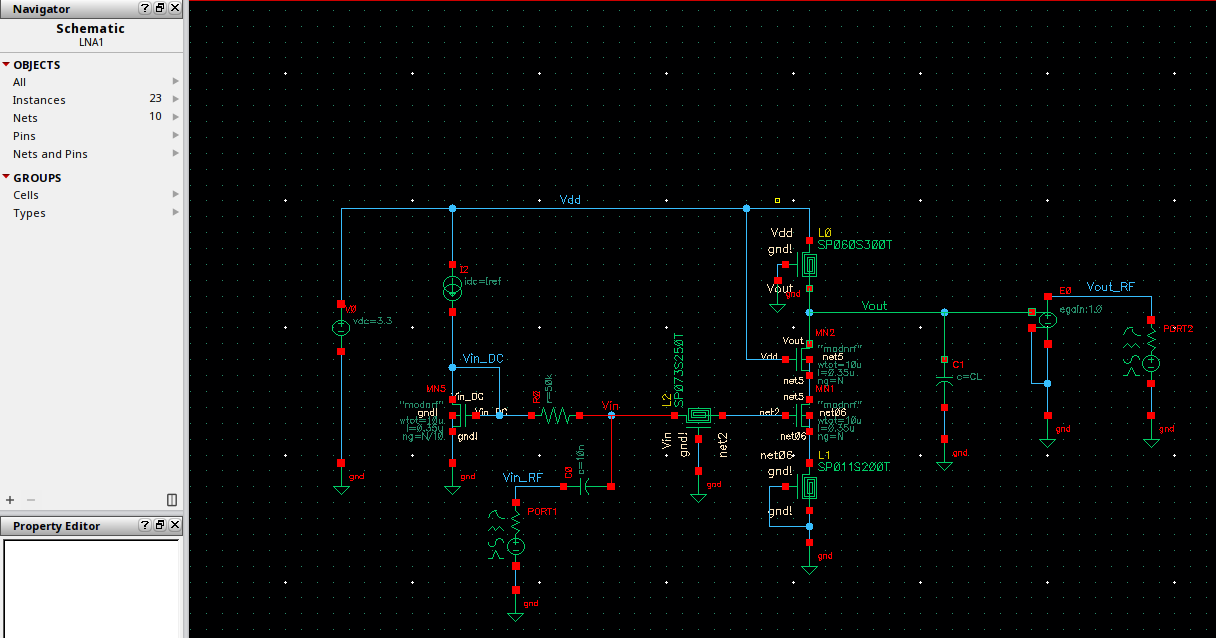
\includegraphics[scale=0.45]{schematic-3-1.png}
   \caption{Schematic}
\end{figure}

\begin{figure} [H] \centering
   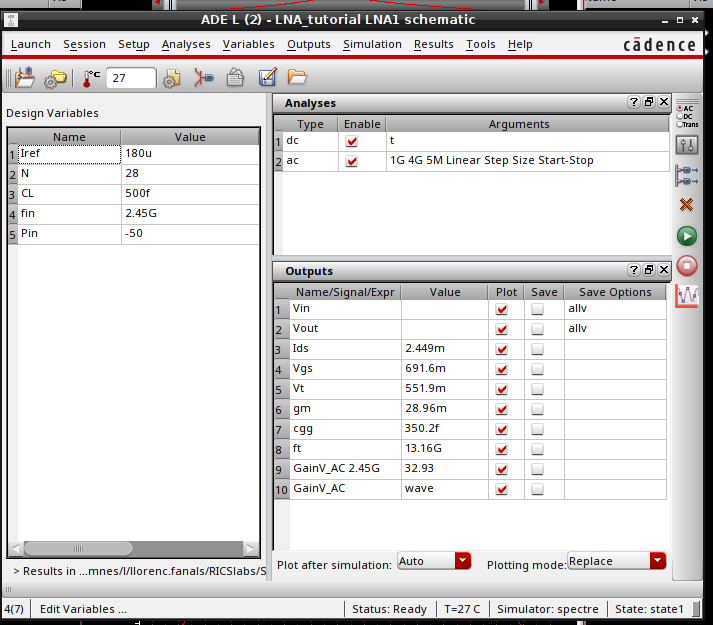
\includegraphics[scale=0.5]{ade-3-1.png}
   \caption{ADE window}
\end{figure}




\begin{pexbox}{}
   \noindent \textbf{Create a small table comparing the OP parameter values against the values expected according to your prelab calculations. Include them in your report.}
\end{pexbox}

   \noindent As commented, I use the numbers provided by the professor, and for $V_{TH}$ I take the value that appears on the technology data table.
   \begin{table}[H] \centering
      \begin{tabular}{ |l|r|r| } \hline
          Characteristic & Theoretical value & Simulation value \\ \hline \hline
          $I_{DC}$ & $2.5$ mA & $2.449$ mA \\ \hline
          $V_{GS}$ & $0.6822$ V & $0.6961$ V \\ \hline  
          $V_{TH}$ & $0.5$ V & $0.5519$ V \\ \hline
          $g_m$ & $24.7$ mA/V & $28.96$ mA/V \\ \hline
          $C_{GG}$ & $350$ fF & $350.2$ fF \\ \hline
          $f_T$  & $11.2$ GHz & $13.16$ GHz \\ \hline
      \end{tabular}
      \caption{Parameter comparison}
   \end{table}
\noindent The results are smilar in most cases. The transconductance $g_m$ is higher for the simulation, thus leading to a higher $f_T$ value, too. This is something positive, we can get a higher gain for the same power consumption.

\begin{pexbox}{}
   \noindent \textbf{Capture the results of the AC analysis, including markers measuring the ressonance frequency and voltage gain.}
\end{pexbox}


\begin{figure} [H] \centering
   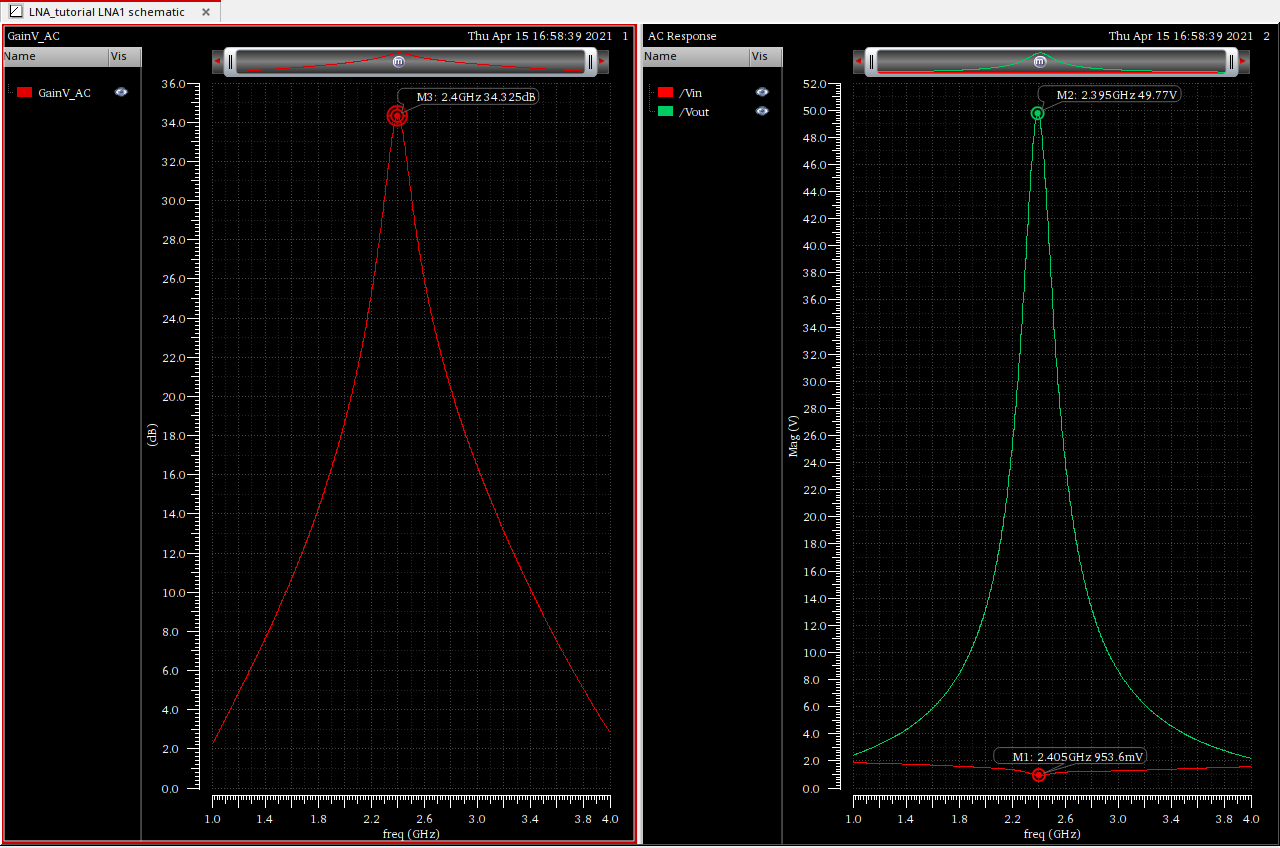
\includegraphics[scale=0.45]{plots-3-2.png}
   \caption{Gain and voltage plots}
\end{figure}

% \noindent From the plots, the ressonant frequency is at $2.4$ GHz. The gain is higher than $30$ dB, which was the gain for which the design was made. This is thanks to the unexpected increase in $g_m$ that appears in the simulation.
\begin{equation}
   |A_v| = 34.325 \text{ dB} \ .
\end{equation}

\begin{pexbox}{}
   \noindent \textbf{Can you extract some information on the input matching, from the plots obtained?}
\end{pexbox}

\noindent I extract that input matching must be very good because the obtained gain is higher than $A_v = 30$ dB, which was the gain we pursued in the pre-lab. Part of this comes from the fact that the $g_m$ obtained is greater than the theoretical one, but in spite of this we wouldn't obtain this large gain if it was not for very good input matching, which is evaluated in the following section.




\section{Evaluating Gains and Input Matching}
\begin{pexbox}{}
   \noindent \textbf{Capture the plot of the S11 parameter, including markers to measure the ressonance frequency of S11 and its value at $f_0 = 2.45$ GHz.}
\end{pexbox}

\begin{figure} [H] \centering
   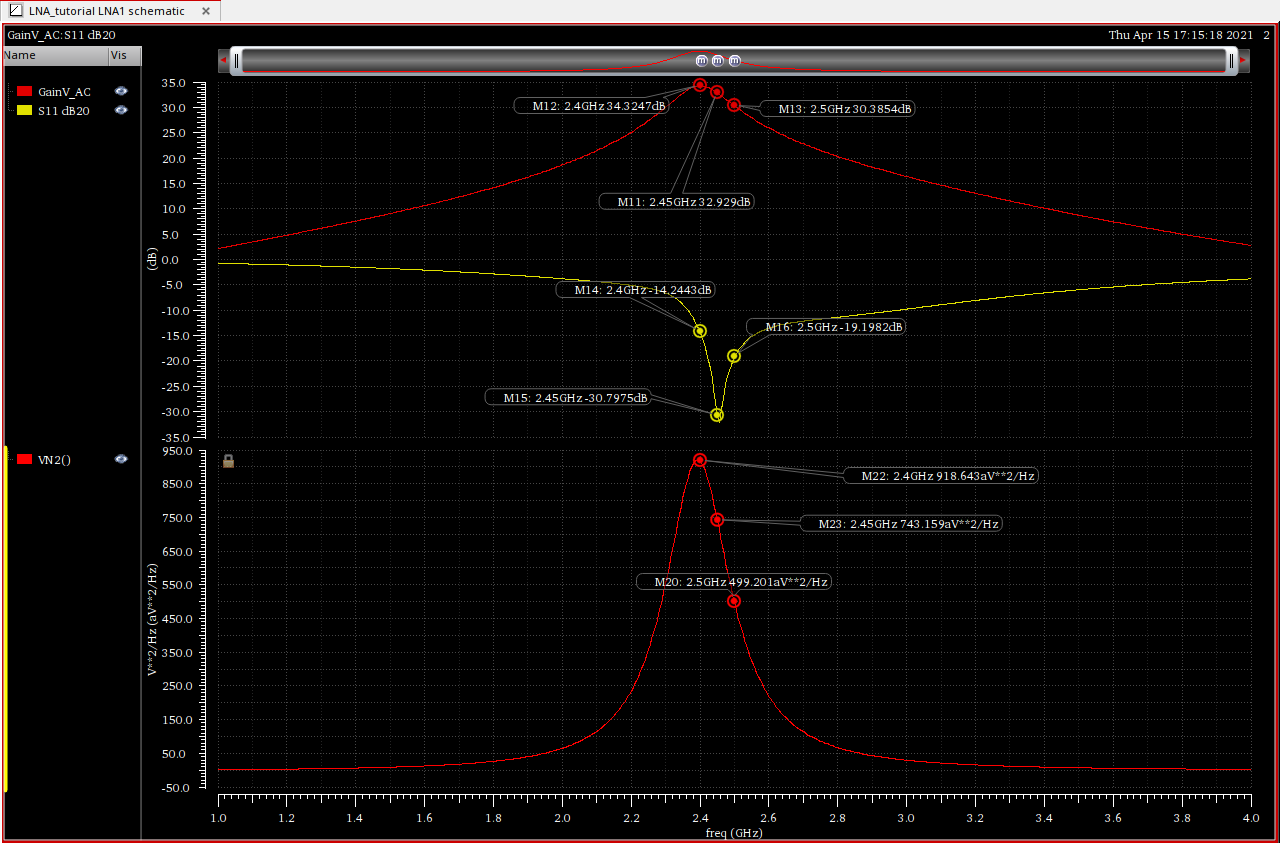
\includegraphics[scale=0.45]{4-2-s11-plots.png}
   \caption{Gain and S11 plots}
\end{figure}

\noindent While $f=2.45$ is not the frequency for which the gain is at its maximum, it is the frequency for which the input matching is best.
\begin{equation}
   S_{11}|_{2.45 \text{ GHz}} = -30.7975 \text{ dB} \ .
\end{equation}
\noindent This fulfils the $S_{11}$ specification without a problem, which consisted on $S_{11} < -10$ dB. 

\noindent Around $f_0$, the central frequency, the S11 parameter shows very small values. This means that the ratio between the reflected wave and the incident wave is very low (if perfectly isolated, as is the case thanks to the buffer, S11 is just this relation). This is something desired because it means that almost no power will be lost in the input stage, so it can be concluded impedance matching is very good. 

\noindent Recall,
\begin{equation}
   \begin{pmatrix}
      V_1^- \\
      V_2^+
   \end{pmatrix} = \begin{pmatrix}
      S_{11} & S_{12} \\
      S_{21} & S_{22} 
   \end{pmatrix} \begin{pmatrix}
      V_1^+ \\
      V_2^-
   \end{pmatrix} \ .
\end{equation}



\begin{pexbox}{}
   \noindent \textbf{Capture the plots of the impedance, including markers at $f_0 = 2.45$ GHz.}
\end{pexbox}
   
   \noindent Now, the input impedance is obtained, both the real and imaginary parts. Recall that, ideally, the imaginary impedance should be $0$ at $f_0$ and the real impedance should be $50 \ \Omega$. The closer to these values, the better.
\begin{figure} [H] \centering
   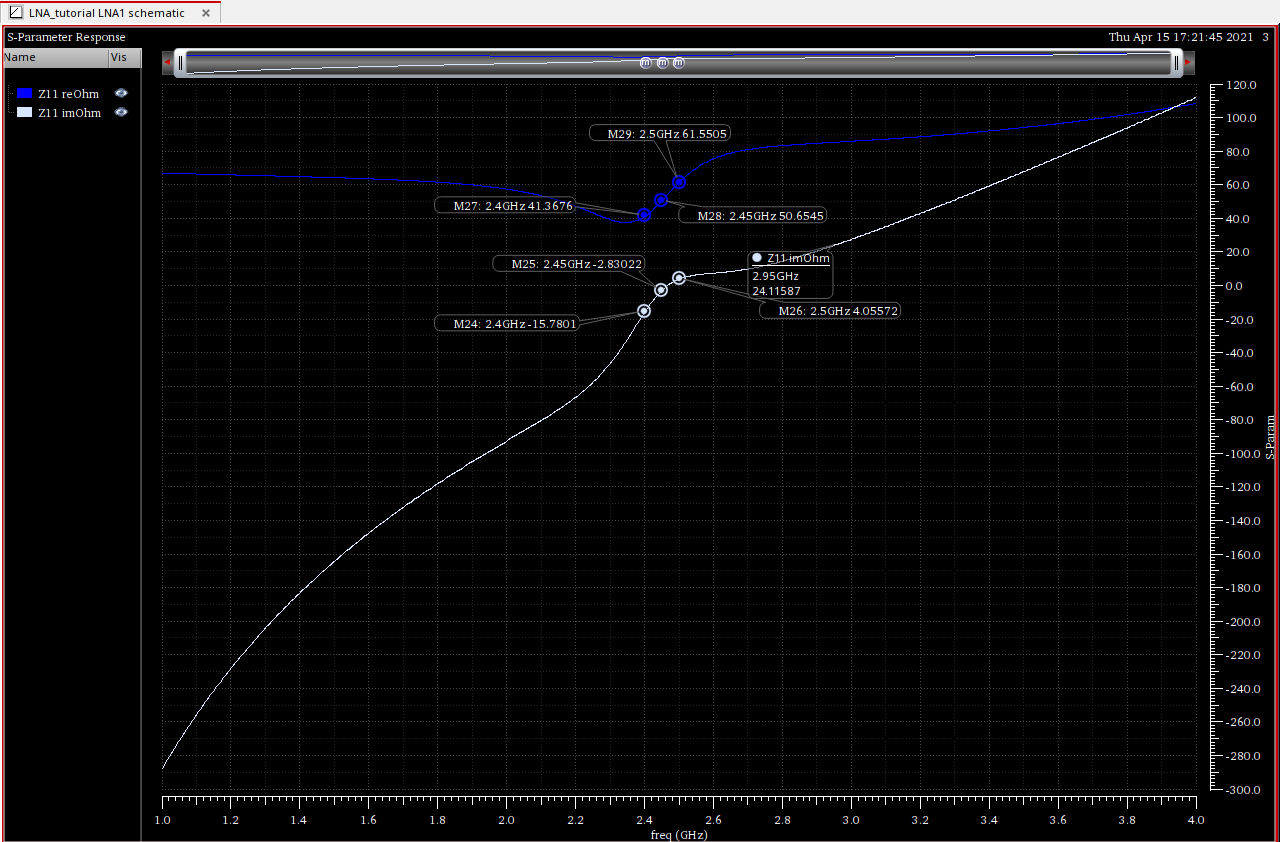
\includegraphics[scale=0.45]{4-2-z11-imag-real.png}
   \caption{Z11 plots}
\end{figure}

\noindent Notice the real impedance at $2.45$ GHz is very close to $50 \ \Omega$, and that the imaginary part is $-2.83022 j \ \Omega$. So, the source impedance is very close to being matched by the amplifier input impedance. This explains the good $S_{11}$ parameter.


\begin{pexbox}{}
   \noindent \textbf{Compare the values obtained, to the targeted ones.}
\end{pexbox}

   \noindent Ideally, the amplifier input impedance should be equal to the voltage source output impedance: a real $50 \ \Omega$. Matching is not perfect but very close to it. By using the professor's numbers, I avoid having to tune the design. I already get a very low S11 parameter and a gain above $30$ dB.


\noindent Also, I've obtained the Smith chart:
\begin{figure} [H] \centering
   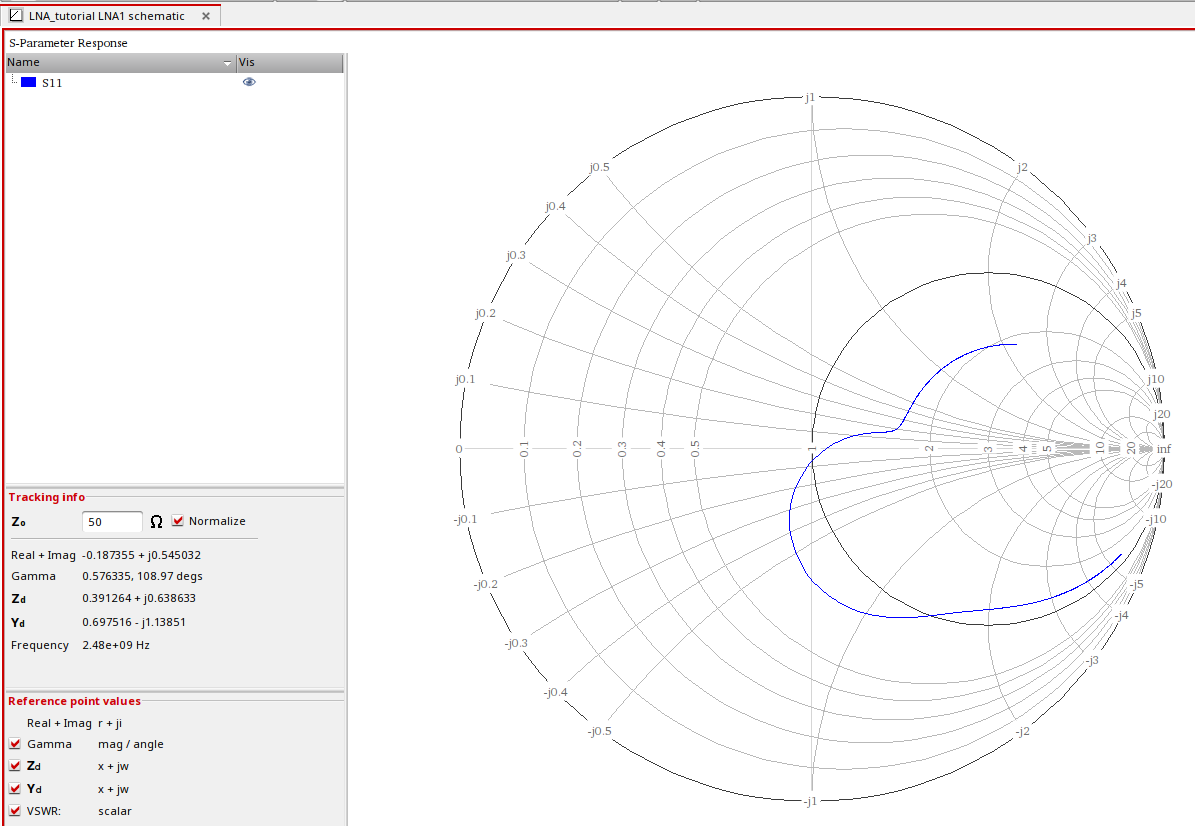
\includegraphics[scale=0.45]{smith.png}
   \caption{Smith chart}
\end{figure}

\noindent Notice the plot, in blue, crosses the unit circle around $-0.05 j$. Considering it is normalized to $50 \ \Omega$, as commented on the laboratory document and as appears in the plot itself, this would lead to $\approx -2.5j$, which is very close to the actual obtained value, $-2.83022 j \ \Omega$. As the cross is not in the center of the plot, matching is not perfect, but it's quite close to it.



\begin{pexbox}{}
   \noindent \textbf{Capture the plots, including markers at $f_0 = 2.45$ GHz.}
\end{pexbox}

   \noindent Now, we are interested in the gain from input to output. Notice from the previous equation that $S_{21}$ relates the $V_2^+$ to $V_1^+$. $V_2^-$ in theory also affects, but in principle $S_{22}$ is very low. The transducer power gain, $G_T$, and the operating power gain $G_P$, are
   \begin{equation}
      \begin{split}
         G_T &= 10 \log \left( \frac{P_{OUT}}{P_A}\right) = 10 \log(|S_{21}|^2) \\
         G_P &= 10 \log \left(\frac{P_{OUT}}{P_{IN}}\right) = G_V + 10 \log \left( \frac{R_{in}}{R_{L}}\right) = 10 \log \left( \frac{|S_{21}|^2}{1 - |S_{11}|^2} \right)
      \end{split} \ .
   \end{equation}
   \noindent If $|S_{11}|$ is very low, which as seen previously is true, and can approximate $S_{11} \approx 0$, then $G_T = G_P$, i.e., the trasducer power gain is equal to the operating power gain. For frequencies far from the ressonant frequency, high differences can be expected between $G_T$ and $G_P$, because $S_{11}$ is not longer approximately $0$, which means that input matching is no longer close to perfection. Next, the $S_{21}$, $G_T$ and $G_P$ plots are shown.

\begin{figure} [H] \centering
   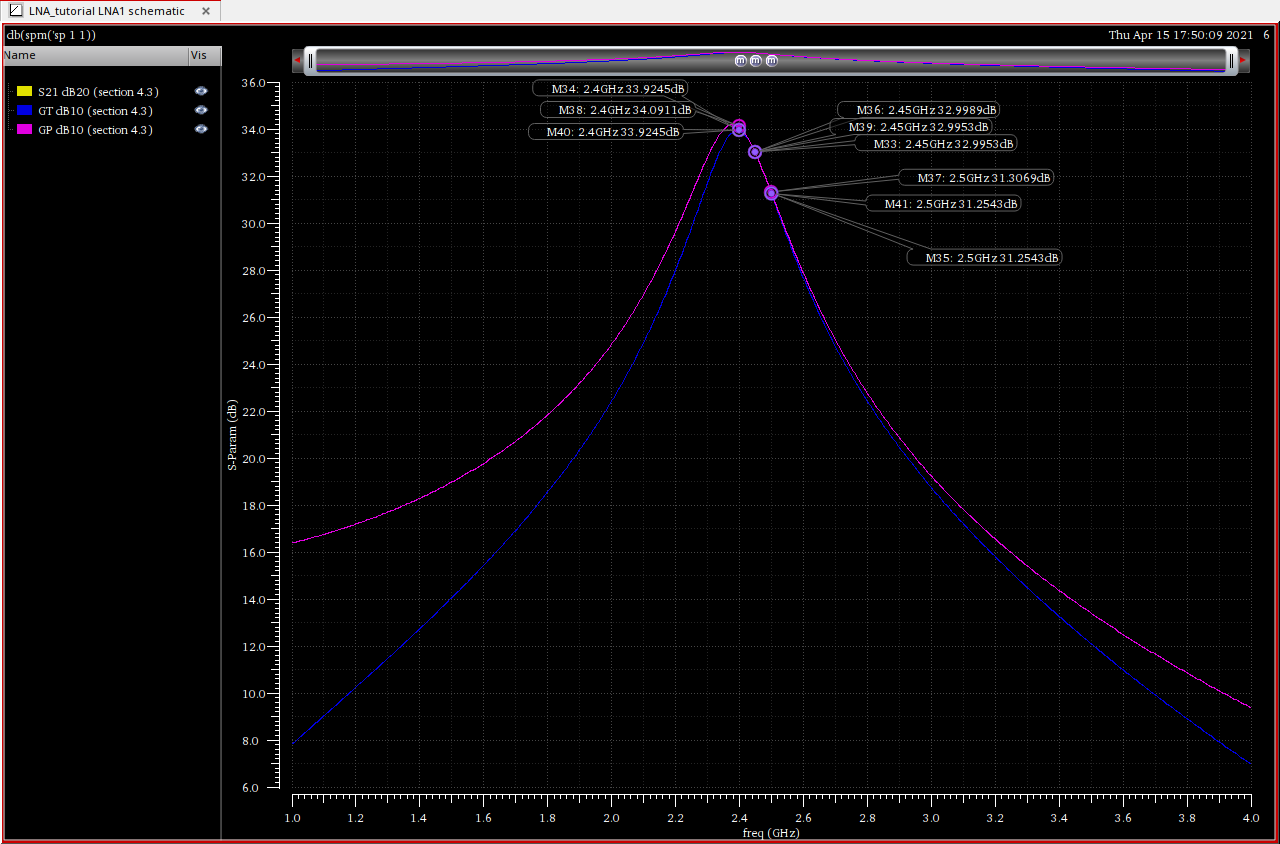
\includegraphics[scale=0.45]{4-3-gs.png}
   \caption{GT, GP, S21 plots}
\end{figure}

\noindent The $S_{21}$ plot is overlapped with the $G_T$ plot. It makes sense according to the definition I've just given. When there is not a good input matching (for frequencies far from the central one), the input power is lower than the one provided by the voltage source and thus $G_P > G_T$, because there's no perfect impedance matching, and thus $P_{IN} < P_{A}$. The $G_P$ resembles a lot the gain plot I showed before. Anyways, the differences between the three plots are minimal in the expected frequencies.


\begin{pexbox}{}
   \noindent \textbf{Are the results obtained consistent with the theoretical expectations?}
\end{pexbox}

\noindent Yes, when there's good input matching (around the central frequency), the gain is over $30$ dB, as desired. And when there's not good input matching, which is something that happens for frequencies far from the central one, the gain is much lower. Also, we know $G_P$ is more "optimistic" than $G_T$; the port component provides the specified power to the amplifier, at the cost that far from the central frequency $P_A$ must be considerably higher than $P_{IN}$, i.e., not all the available power at the source arrives at the input of the amplifier.




   \noindent Now, I've changed the PORT2 impedance to $500 \ \Omega$. Keep in mind the original schematic: the output port, PORT2, was connected to a 4-port component that copied the voltage at its two input ports to its two output ports, i.e., a simple buffer. So, the gain shown by the amplifier itself, defined as the output voltage divided by the input voltage, should not change in spite of increasing the output impedance. 


\begin{pexbox}{}
   \noindent \textbf{Measure the four gain values at $f_0 = 2.45$ GHz.}
\end{pexbox}

\begin{figure} [H] \centering
   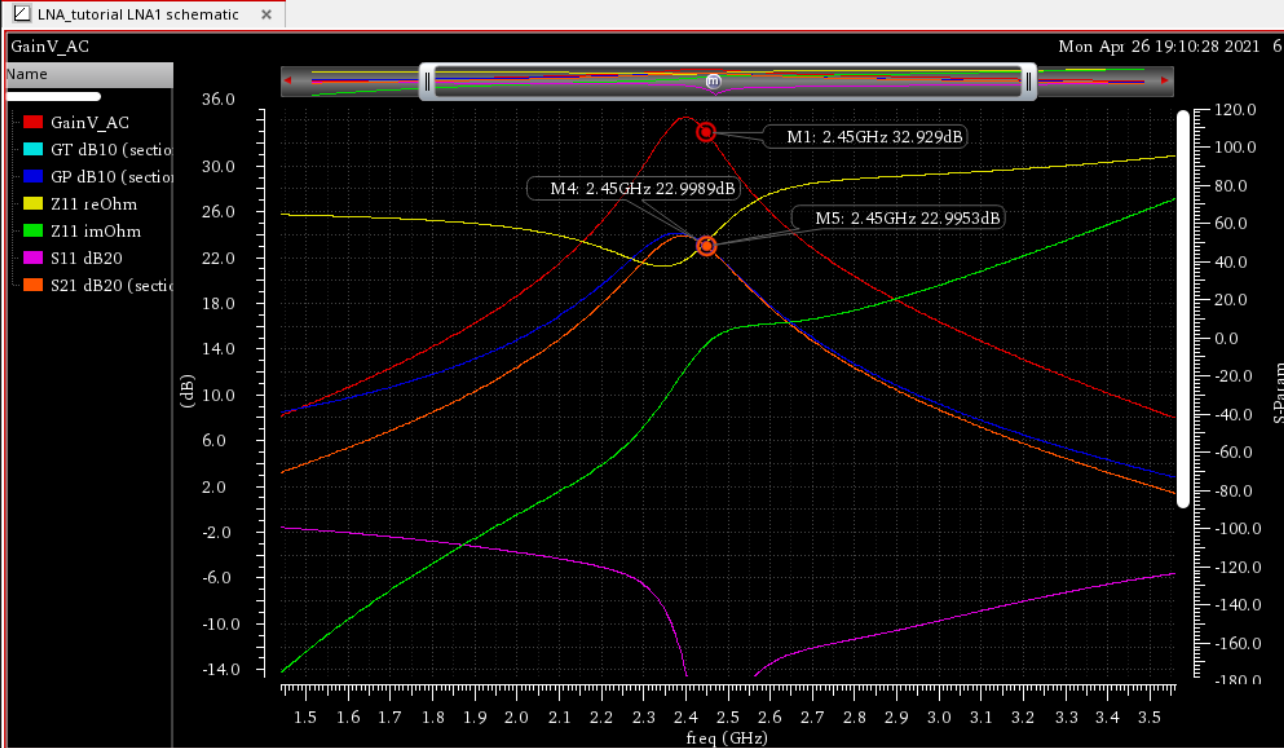
\includegraphics[scale=0.45]{4-3-500ohm.png}
   \caption{Plots}
\end{figure}

\noindent Again, the $S_{21}$ plot is overlapped to the $G_T$.

\begin{pexbox}{}
   \noindent \textbf{Are the results obtained consistent with the theoretical expectations?}
\end{pexbox}

\noindent By increasing the output impedance by a $10$ factor, the $10 \log \left( \frac{R_{in}}{R_{L}}\right)$ term decreases by $10$ dB. This happens to $G_P$, clearly from the equation, and also to $|S_{21}|$ and thus $G_T$. This is the reason for the $10$ dB shift.




\begin{pexbox}{}

   \noindent Next, I've added a $100 \ \Omega$ series resistance with $L_G$.

   \noindent \textbf{Capture the plots of the four gains, and the S11 parameter, including markers at $f_0 = 2.45$ GHz.}
\end{pexbox}


\begin{figure} [H] \centering
   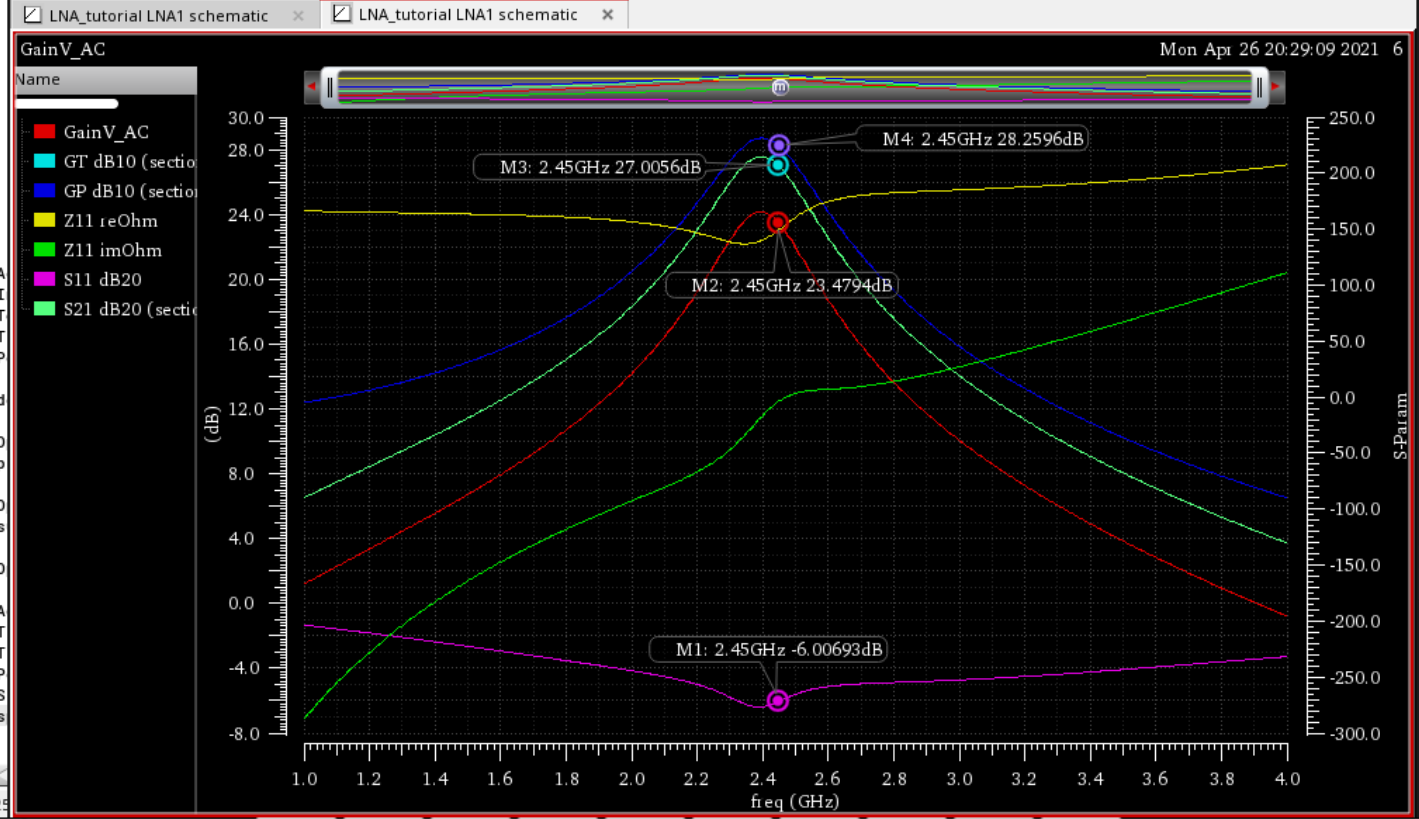
\includegraphics[scale=0.4]{4-3-100ohm.png}
   \caption{Plots}
\end{figure}

\noindent Again, the $S_{21}$ plot is overlapped to the $G_T$.

\begin{pexbox}{}
   \noindent \textbf{Are the results obtained consistent with the theoretical expectations?}
\end{pexbox}
   
\noindent Now, there's no input matching at the central frequency. Recall we've verified our circuit was quite good at showing a real $50 \ \Omega$ input impedance at $f_0$. Now, by adding a resistance of $100 \ \Omega$ in series with the gate inductance, clearly $S_{11}$ won't be as low as before, meaning there will be a partial reflection at the input and thus the output power will be lower. At the same time, this will mean the output gain will be lower.

\noindent Before, it was shown that we had $S_{11} = -30.7975$ dB. Now, this is just $-6$ dB. For the $G_V$ gain, I notice the linear factor between the previous gain and the current one is very close to $3$. It makes sense if one considers that only $1/3$ of the voltage at the input node reaches the circuit we had before, i.e., $2/3$ of voltage fall at the $100 \ \Omega$ resistance. 

\noindent $G_T$ and $G_P$ also result affected by this. From previous expressions, it can be seen that $G_T - 10 \log(1 - |S_{11}|^2) = G_P$. The plotted $S_{11}^2 = -6 \text{ dB} = 0.2512$, so $10 \log(1- |S-{11}|^2) = 0.7488 = -1.256$ dB, which is almost exactly the difference $G_P - G_T$. The $G_P$ gain has also been reduced $-6$ dB from its original value, because of bad input matching.  
% revisar 4port components i justficiar els GT i GP





\section{Evaluating Isolation and Stability}
\begin{pexbox}{}
   \noindent \textbf{Capture the plot evaluating the reverse isolation, including marker at $f_0 = 2.45$ GHz.}
\end{pexbox}

\begin{figure} [H] \centering
   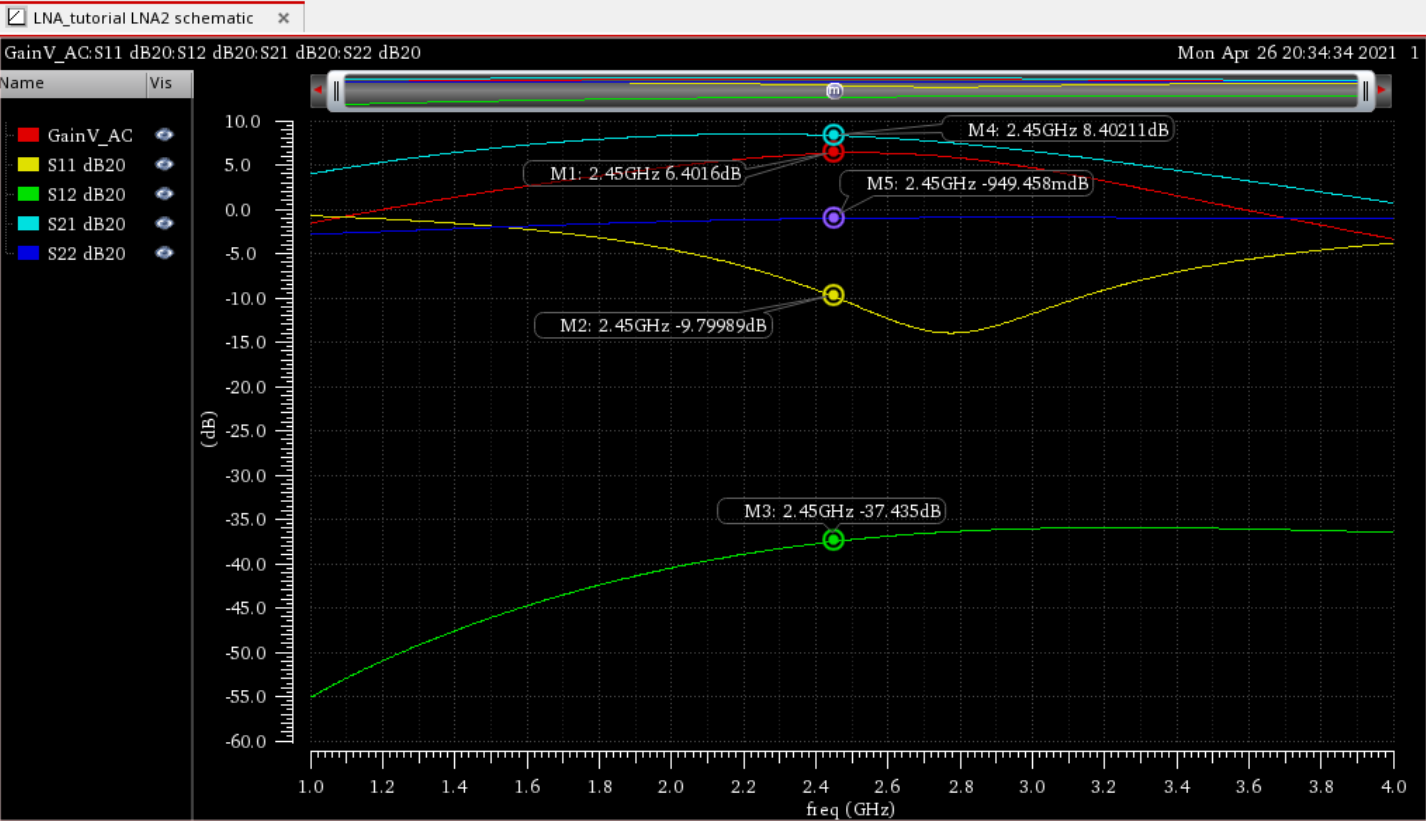
\includegraphics[scale=0.4]{5-2.png}
   \caption{S parameters and gain plots}
\end{figure}


\begin{pexbox}{}
   \noindent \textbf{Does the reverse isolation have a good value?}
\end{pexbox}

   \noindent Although it could always be lower, in a linear scale $S_{12} \approx 0.014$, so the contribution to $V_{1}^-$ by the output is almost "only" $1$\% of the output voltage. However, keep in mind the output voltage is amplificated by around $30$ dB (in fact, from simulations it was around $33$ dB). So, the input voltage is amplified by the amplifier, and then part of this amplified signal is fedback to the input. The fedback signal is $\approx -4$ dB with respect to the input signal.
   
   \noindent We already have the cascode transistor that helps quite a lot in isolating the output and the input (mainly the Miller capacitance that would appear with a single transistor does not longer appear with the cascode). So, I don't think there's much more to do to improve the $S_{12}$ parameter. Keep in mind the comment made in the document lab, it suggests that this output loading would not happen in a real situation, so we should not bother much about it.




\begin{pexbox}{}
   \noindent \textbf{Also, check the consistency of the other S-parameters.}
\end{pexbox}

   \noindent I think the $S_{11}$ is not as low as before, but in the beginning we were required to get $S_{11}<-10$ dBm, and in this case I almost get it. Impedance matching could be better, but it's decent. Of course, $S_{21}$ shows the higher values.



\begin{pexbox}{}
   \noindent \textbf{Capture the plots of stability parameters, including markers at minimum/maximum values.}
\end{pexbox}

\begin{figure} [H] \centering
   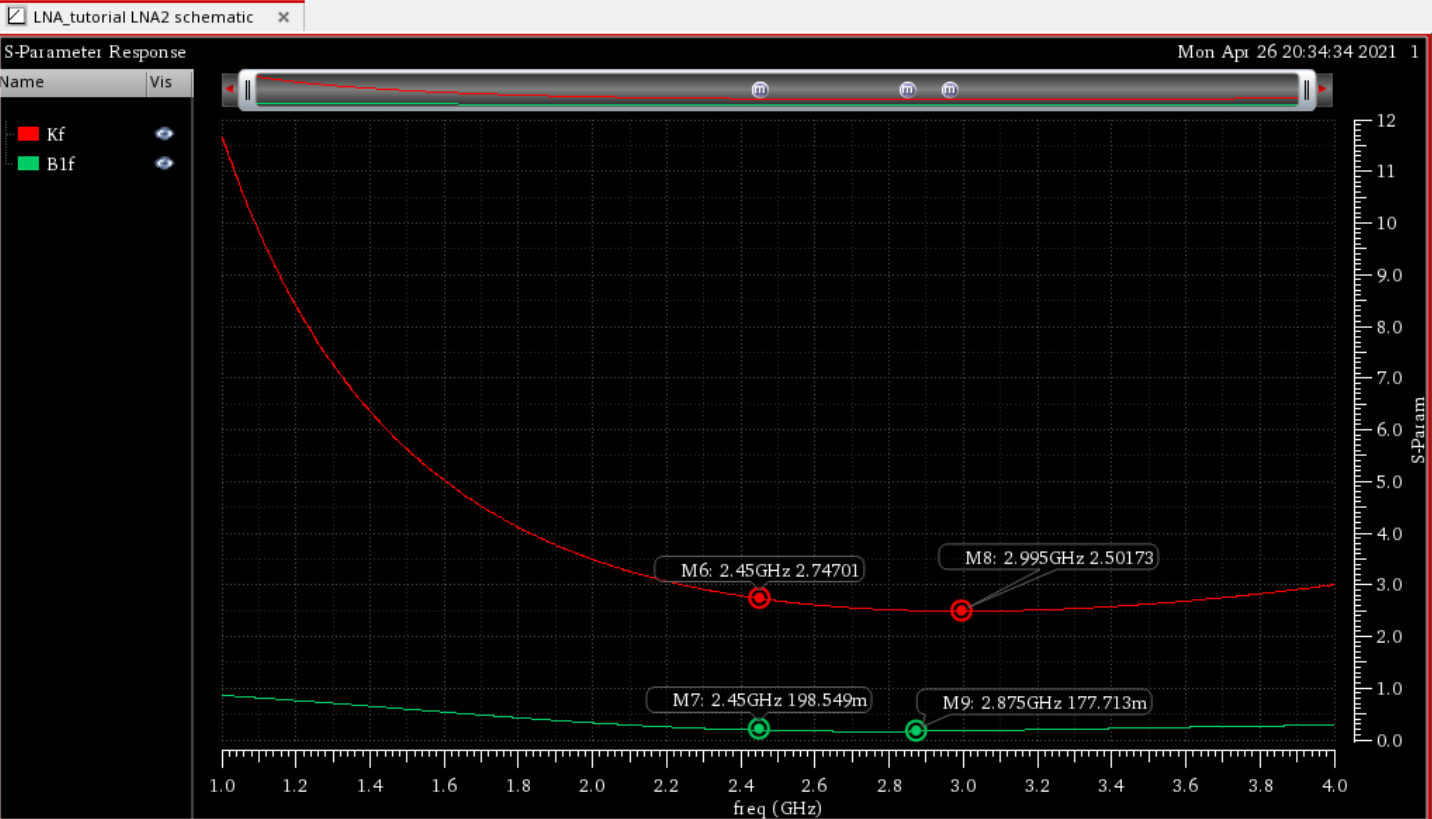
\includegraphics[scale=0.4]{5-3.png}
   \caption{Stability parameters plots}
\end{figure}


\begin{pexbox}{}
   \noindent \textbf{Is the LNA unconditionally stable?}
\end{pexbox}

   \noindent Yes, according to the conditions $K_f>1$ and $B_{1f}>0$.
 


\section{Evaluating Noise performance}
\begin{pexbox}{}
   \noindent \textbf{Capture the plots of NF obtained, including markers at $f_0 = 2.45$ GHz.}
\end{pexbox}
   
   \noindent I've obtained the Noise Figure, NF, from ADE - Results - Direct Plot - Noise Figure, without using the Direct Plot.
\begin{figure} [H] \centering
   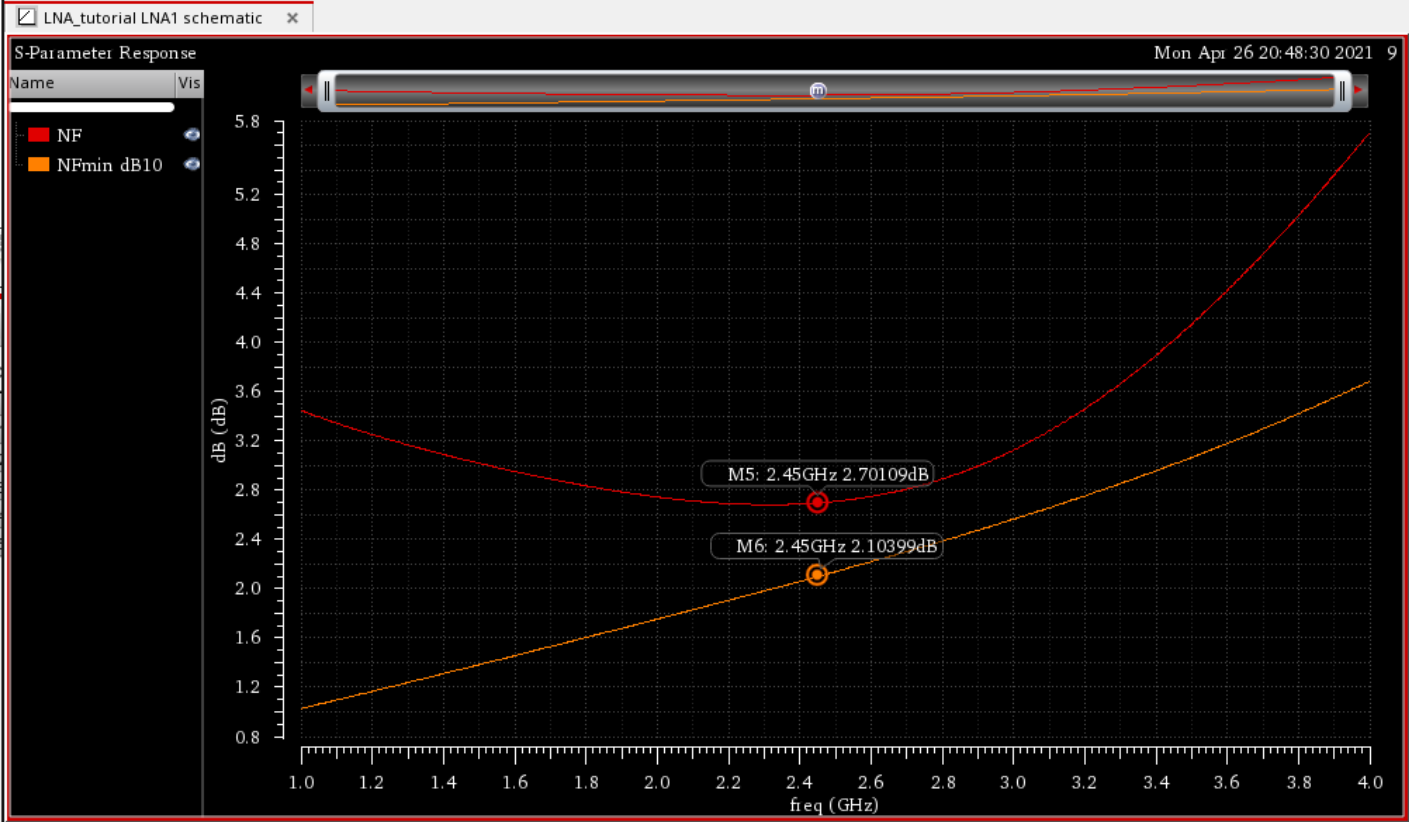
\includegraphics[scale=0.4]{6-1.png}
   \caption{NF plots}
\end{figure}


\begin{pexbox}{}
   \noindent \textbf{Is the NF close to the value theoretically expected?}
\end{pexbox}
   
   \noindent The theoretical value, with the professor's numbers, is
   \begin{equation}
      NF = 2.6 = 4.15 \text{ dB} \ .
   \end{equation}
   \noindent This doesn't fulfill the desired NF, $NF < 3$ dB, but in the pre-lab we were told we could fix this by increasing the current consumption to increase $f_T$. 
   
   \noindent However, after the simulation, the obtained NF is better than the theoretical one, and it fulfills $NF < 3$ dB.

\begin{pexbox}{}
   \noindent \textbf{Does the LNA fulfill the targeted NF specification?}
\end{pexbox}

   \noindent As commented, yes. As commented in the lab, this analysis tends to be optimistic, as it is done after linearizing the equations. If a large-signal analysis was performed, NF would tend to be worse (larger).




\begin{pexbox}{}
   \noindent \textbf{Capture the (upper part of the) Noise Summary window.}
\end{pexbox}

\begin{figure} [H] \centering
   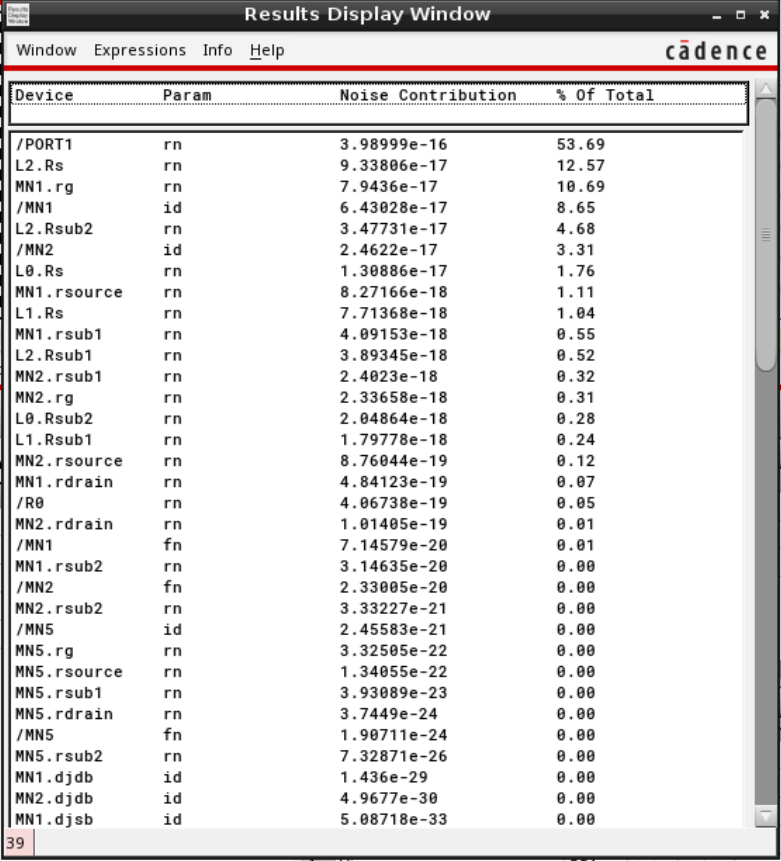
\includegraphics[scale=0.5]{6-2.png}
   \caption{Noise summary}
\end{figure}


\begin{pexbox}{}
   \noindent \textbf{Identify the noise sources that contribute more than 5\% to the total noise.}
\end{pexbox}

   \noindent As can be seen from the figure, only $4$ noise sources contribute more than $5$\% to the total noise. It's required to understand their origin.
   \begin{equation}
      \begin{split}
         /PORT1 &:  \text{Input voltage source 50 $\Omega$ equivalent resistance} \\
         L2.Rs &:  \text{Gate inductance series resistor} \\
         MN1.rg &:  \text{Input NMOS equivalent gate resistance} \\
         MN1 &:  \text{Input NMOS channel noise} \\
      \end{split} \ .
   \end{equation}

\begin{pexbox}{}
   \noindent \textbf{What does it mean that noise of PORT1 contributes more than 50\%?}
\end{pexbox}

   \noindent That the majority of the noise at the output comes from the input equivalent circuit, and thus that the LNA noise contribution is lower than the source one. The $NF=2.7$ dB is equal to $1.365$ in linear units. Recall
   \begin{equation}
      F = 1 + \frac{R_{Lg}}{R_s} + \frac{R_{Rg}}{R_s} + \frac{\gamma}{\alpha} g_m R_s \left(\frac{w_0}{w_T}\right)^2 \ .
   \end{equation}
   \noindent And we normally used
   \begin{equation}
      F_{min} = 1 + \frac{R_{Lg}}{R_s} + \frac{R_{Rg}}{R_s} + 2.4 \frac{\gamma}{\alpha} \frac{w_0}{w_T} \ .
   \end{equation}
   \noindent In our analysis, we neglected the NMOS equivalent gate resistance contribution. In the pre-lab, we had $R_{Lg} = 16 \ \Omega$. We calculated $f_T = 11.2$ GHz and we were given $\gamma = 2$, $\alpha = 0.8$. This lead us to $F = 2.6$. 

\begin{pexbox}{}
   \noindent \textbf{Is the contribution of the gate inductor $L_G$ larger of smaller than that calculated?}
\end{pexbox}

   \noindent Now, we have
   \begin{equation}
      \frac{R_{Lg}}{R_s} = \frac{L2.Rs}{/PORT1} = 0.234 \ .
   \end{equation}
   \noindent Before, with $R_{Lg} = 16 \ \Omega$, $\frac{R_{Lg}}{R_s} = 0.32$. So, the gate inductor contribution is lower, now.



\begin{pexbox}{}
   \noindent \textbf{Is the contribution of the channel thermal noise larger of smaller than that calculated?}
\end{pexbox}

   \noindent Now, we have
   \begin{equation}
       2.4 \frac{\gamma}{\alpha} \frac{w_0}{w_T} = \frac{MN1}{/PORT1} = 0.16 \ .
   \end{equation}
   \noindent While before this term was $\frac{\gamma}{\alpha} \frac{w_0}{w_T} = 1.267$. So, the simulation attributes less noise to the channel than the one we calculated. It helps that $w_T$ is greater than in the pre-lab calculations, as shown in a table before. The low channel termal noise is the main source of noise improvement.
   % segur?


% unitats del summary son V^2, canvia algo aixo???

\begin{pexbox}{}
   \noindent \textbf{Is the value of the gate resistance coherent with the contribution to the total output noise? Justify your answer}
\end{pexbox}

\noindent The gate resistance value I get is $R_g = 10.63 \ \Omega$.
\begin{figure} [H] \centering
   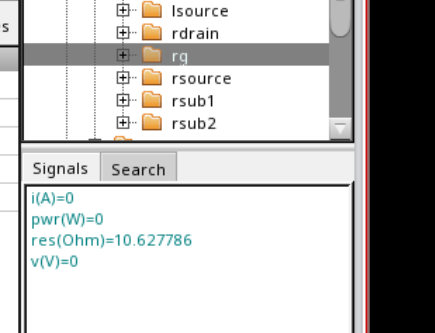
\includegraphics[scale=0.45]{6-rg.png}
   \caption{$R_g$ value at the CS transistor}
\end{figure}
\noindent So, it's contribution to the total noise should be $\frac{R_g}{R_s} = \frac{10.63}{50} = 0.2126$, normalized to the source noise (/PORT1). In the noise summary, the relation is $\frac{10.69}{53.69} = 0.199$. So, the value of the gate resistance is coherent with the contribution to the total output noise.


\begin{pexbox}{}
   \noindent \textbf{Optional: You can try to improve the NF by decreasing the gate resistance. We know this resistance can be reduced by layout, i.e. decreasing the finger size (and increasing the number of fingers, to preserve the total width).}
\end{pexbox}

\noindent I've decreased from $10$ to $5$ the stripe width, and instead of $N$ now I've set $2N$. A small decrease of noise results.
\begin{figure} [H] \centering
   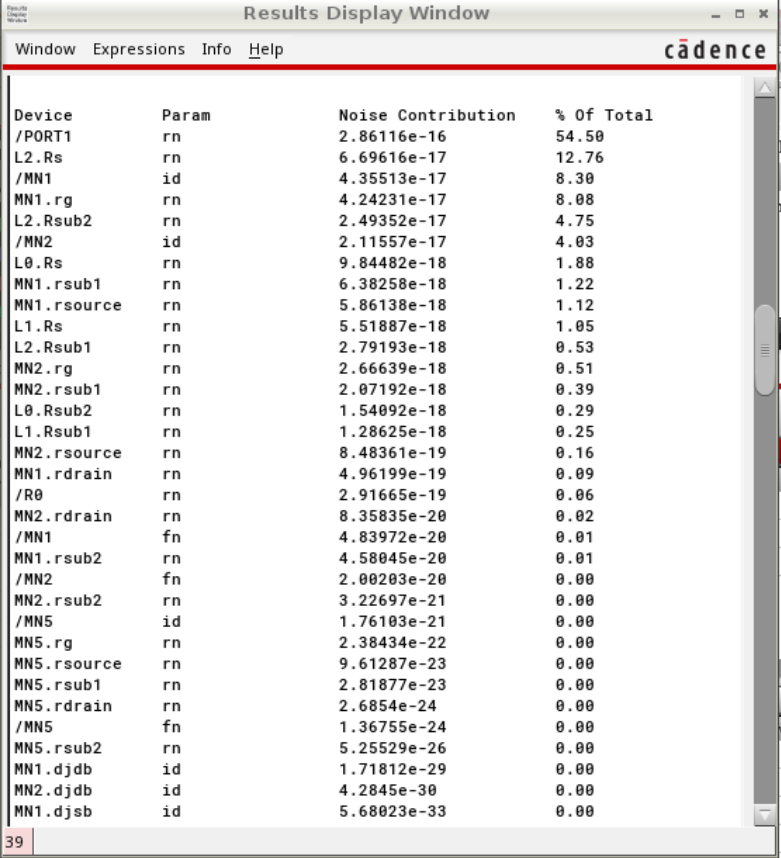
\includegraphics[scale=0.45]{6-2v2.png}
   \caption{Noise summary}
\end{figure}
\noindent Now the contribution from the gate resistance is the previous noise by a factor of $\approx 0.534$, so the improvement is noticeable. Still, in both cases the contribution is quite small overall, so there's not a huge impact on the total noise.





\section{Evaluating Linearity}

\begin{pexbox}{}
   \noindent \textbf{Capture the plot generated for the measurement of IP3.}
\end{pexbox}

\begin{figure} [H] \centering
   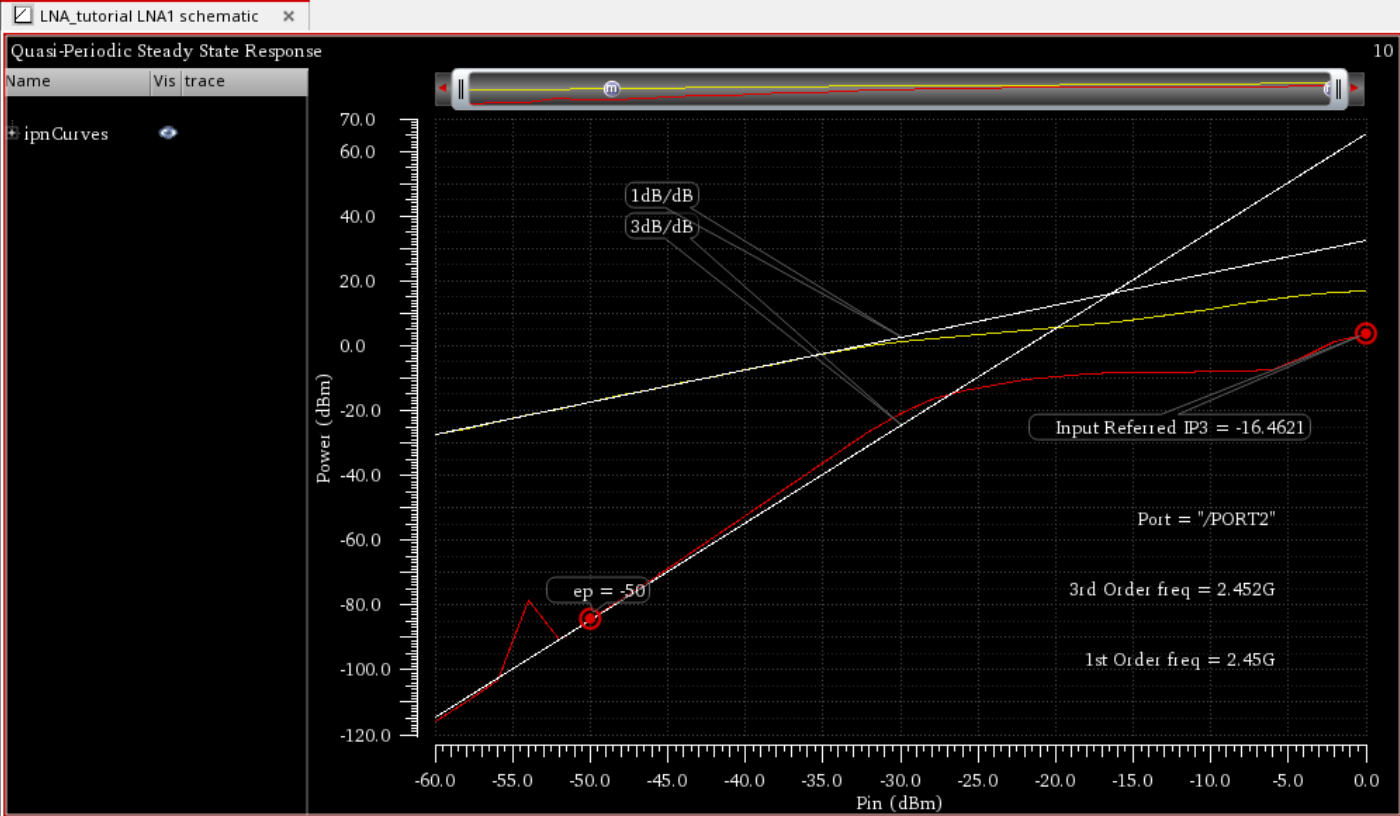
\includegraphics[scale=0.3]{7v0205.png}
   \caption{IP3 analysis}
\end{figure}


\begin{pexbox}{}
   \noindent \textbf{Which is the input-referred IP3 of your LNA?}
\end{pexbox}

   \noindent I get
   \begin{equation}
     % IIP3 = -2.36571 \text{ dBm} \ .
     IIP3 = -16.4621 \text{ dBm} \ .
   \end{equation}

\begin{pexbox}{}
   \noindent \textbf{Which is the OIP3?}
\end{pexbox}

   \noindent Taking the previous $A_v = 33$ dB, I would have
   \begin{equation}
      % OIP3 = 30.634 \text{ dBm} \ .
      OIP3 = 16.54 \text{ dBm} \ .
   \end{equation}
   \noindent This value can be, more or less, deduced on the previous plot, in the vertical axis.

\begin{pexbox}{}
   \noindent \textbf{Which other frequencies you could have selected for the fundamental tone and for the 3rd-order intermodulation product?}
\end{pexbox}

   \noindent The chosen frequencies, $f_1 = 2.45$ GHz and $f_2 = 2.451$ GHz result in third-order tones at $2.452$ GHz and $2.448$ GHz, and thus I've chosen $2.45$ GHz as the $1^{st}$ order harmonic, and $2.452$ GHz as the $3^{rd}$ order harmonic. I could have also chosen $2.451$ GHz as the $1^{st}$ order harmonic, and $2.449$ GHz as the $3^{rd}$ order harmonic, because the two input tones are of the same power, and the tone at $2.449$ GHz will be equal to the one at $2.451$ GHz. I've noticed that for this, the results were almost identical.







\begin{pexbox}{}
   \noindent \textbf{Capture the plot generated for the measurement of CP1dB.}
\end{pexbox}

\begin{figure} [H] \centering
   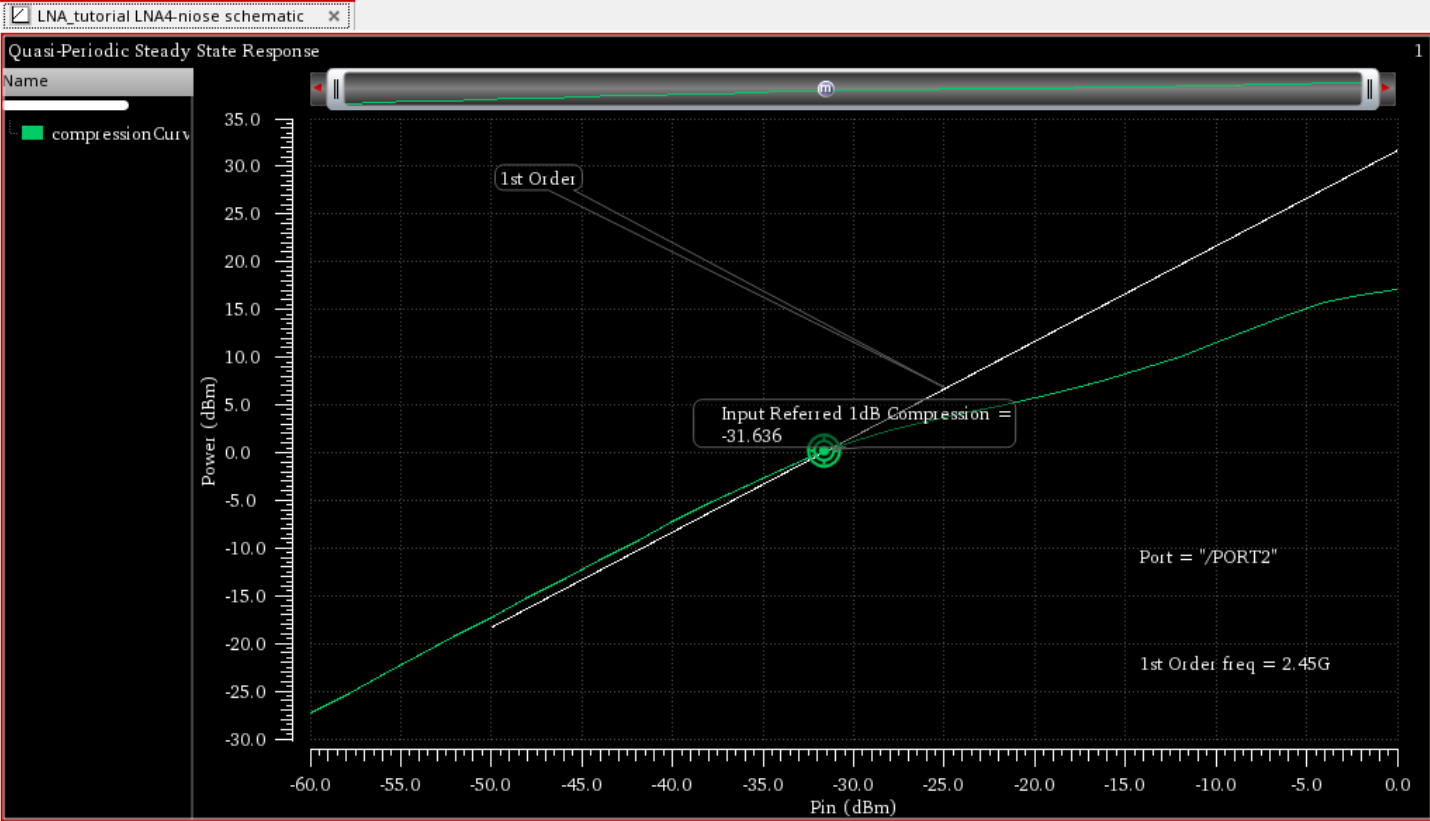
\includegraphics[scale=0.3]{7-comp-0205.png}
   \caption{Compression analysis}
\end{figure}


\begin{pexbox}{}
   \noindent \textbf{Which is the input-referred 1dB Compression point of your LNA?}
\end{pexbox}

   \noindent I get
   \begin{equation}
      P_{in,-1dB} = -31.636 \text{ dBm} \ .
   \end{equation}


\begin{pexbox}{}
   \noindent \textbf{Which is peak input amplitude that corresponds to this CP1dB?}
\end{pexbox}

\noindent By recalling that 
\begin{equation}
   P [dBm] = 10 \log\left(\frac{\frac{(V_{peak}/\sqrt{2})^2}{50}}{1 \text{ mW}}\right) \ ,
\end{equation}
\noindent I get
\begin{equation}
   V_{in,peak,-1dB} = 8.283 \text{ mV}_{peak} \ .
\end{equation}

\begin{pexbox}{}
   \noindent \textbf{Which is the output-referred 1dB Compression point of your LNA?}
\end{pexbox}
%
   \begin{equation}
      P_{out,-1dB} = 1.364 \text{ dBm} \ .
   \end{equation}


\begin{pexbox}{}
   \noindent \textbf{Which is peak output amplitude that corresponds to this CP1dB?}
\end{pexbox}

   \noindent A similar calculation to the one before is performed. I get
   \begin{equation}
      V_{out,peak,-1dB} = 0.370 \text{ V}_{peak} \ .
   \end{equation}









\begin{pexbox}{}
   \noindent \textbf{Optional: it is interesting that you repeat the 1dB compression point representation, but now selecting Power Gain as the output format representation. This provides an alternative interpretation of the 1dB compression point. At small input power, the gain is constant, and the 1dB compression point is the power at which the gain is reduced 1dB.}
\end{pexbox}

\begin{figure} [H] \centering
   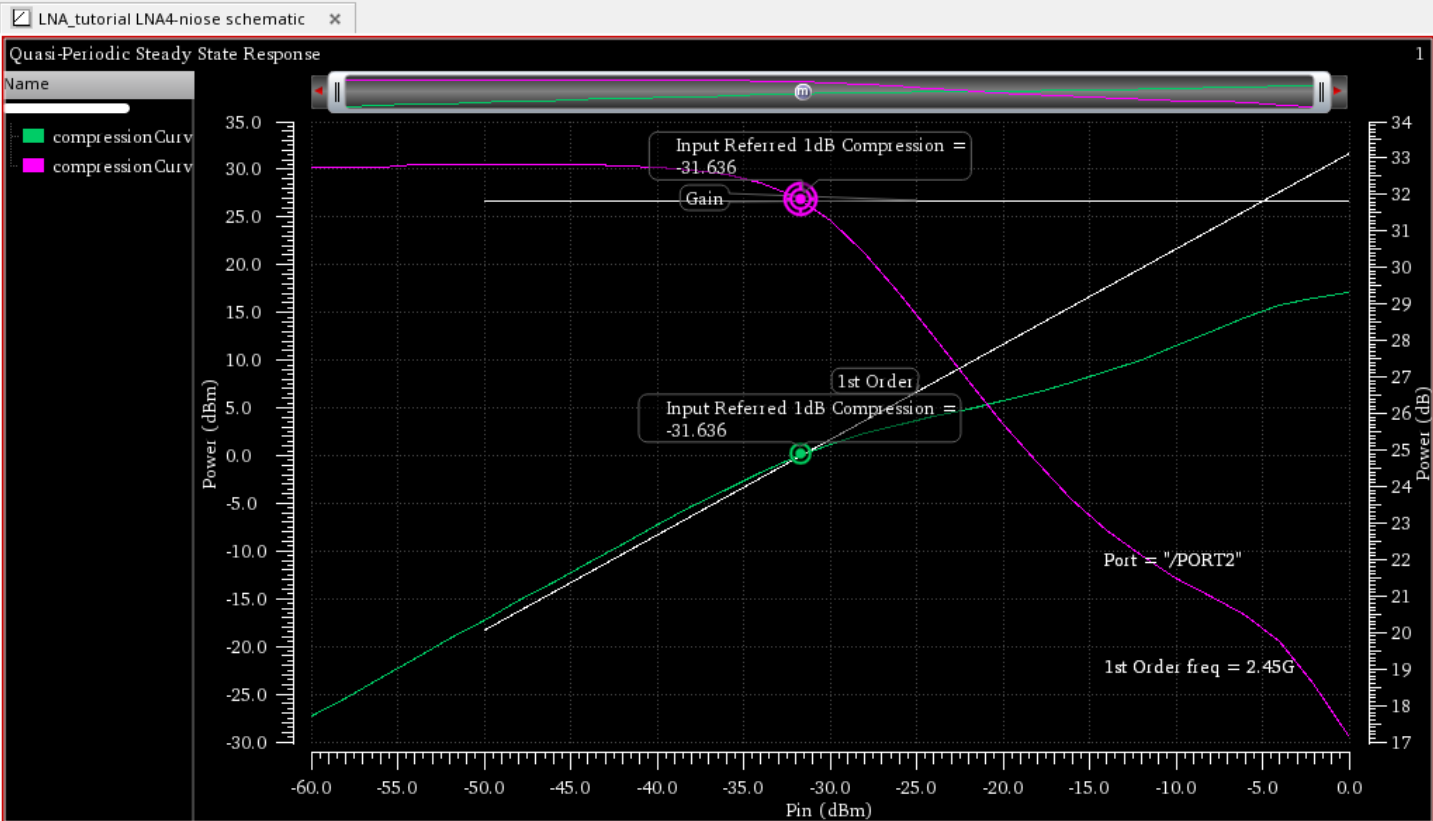
\includegraphics[scale=0.3]{7-compout-0205.png}
   \caption{Compression analysis}
\end{figure}


\noindent I have done it and the resulting plot is more or less as the statement says. For low input powers the response is more or less flat, and for high inputs compression starts taking place and the gain diminishes. The marked compression point is the same as before.




\section{Performance Summary}
\begin{pexbox}{}
   \noindent \textbf{Report the final performance results obtained, fulfilling the next table:}
\end{pexbox}

\noindent I've obtained different $S_{21}$ values during this lab. Some were obtained when there were mismatches, or when the buffer was deleted. We are told "LNA output voltage will drive the input of an on-chip mixer, thus LNA output impedance is not intended to be matched", so it makes more sense to take the first $S_{21}$ I obtained.
\begin{table}[H] \centering
   \begin{tabular}{ |l|r| } \hline
       Characteristic & Value \\ \hline \hline
       Central frequency $f_0$ & $2.45$ GHz \\ \hline % $\approx 2.4$ GHz, designed for 
       S21 (dB) & $32.9953$  \\ \hline % amb buffer, sino 8.4 dB...
       NF & $2.70109$ dB \\ \hline
       IIP3 (dBm) & $-16.4621$ \\ \hline
       Input - CP 1dB (dBm) & $-31.636$ \\ \hline
       S11 (dB) &  $-9.80$ \\ \hline
       Reverse Isolation, S12 (dB) & $-37.435$ \\ \hline
       VDD & $3.3$ V \\ \hline
       IDC (mA) & $2.629$ \\ \hline
       Power Dissipation (mW) & $8.6757$ \\ \hline
       Technology Process & C35B4M3, $0.35 \ \mu$m \\ \hline
   \end{tabular}
   \caption{Final performance results}
\end{table}


% \begin{table}[H] \centering
   % \begin{tabular}{ |l|r| } \hline
       % Characteristic & Value \\ \hline \hline
       % Central frequency $f_0$ & $2.45$ GHz \\ \hline % $\approx 2.4$ GHz, designed for 
       % S21 (dB) & $32.9953$  \\ \hline % amb buffer, sino 8.4 dB...
       % NF & $2.70109$ dB \\ \hline
       % IIP3 (dBm) & $-2.36571$ \\ \hline
       % Input - CP 1dB (dBm) & $1.13416$ \\ \hline
       % S11 (dB) &  $-9.80$ \\ \hline
       % Reverse Isolation, S12 (dB) & $-37.435$ \\ \hline
       % VDD & $3.3$ V \\ \hline
       % IDC (mA) & $2.629$ \\ \hline
       % Power Dissipation (mW) & $8.6757$ \\ \hline
       % Technology Process & C35B4M3, $0.35 \ \mu$m \\ \hline
   % \end{tabular}
   % \caption{Final performance results}
% \end{table}
% quan trec el buffer baixa molt el S21, suposo que es desperar, pero tant petit...

\begin{pexbox}{}
   \noindent \textbf{Optional: You may want to compare the LNA performance you obtained against the performance of LNA designed by international research groups, published in research journals of congresses. A fair comparison would restrict to LNAs designed in similar technology nodes, similar central frequencies, single-ended topologies. We propose eg. the following works:}
\end{pexbox}

\begin{table}[H] \centering
   \begin{tabular}{ |l|r|r|r| } \hline
       Characteristic & LNA lab & Song & Shaeffer \\ \hline \hline
       Central frequency $f_0$ & $2.45$ GHz & $2.1$ GHz & $1.5$ GHz \\ \hline % $\approx 2.4$ GHz, designed for 
       S21 (dB) & $32.9953$ & $16.4$ & $22$  \\ \hline % amb buffer, sino 8.4 dB...
       NF & $2.70109$ dB & $2.77$ dB & $3.5$ dB \\ \hline
       IIP3 (dBm) & $-16.4621$ & $7.45$ & $-9.3$ \\ \hline
       Input - CP 1dB (dBm) & $-31.636$ & - & $-22$  \\ \hline
       S11 (dB) &  $-9.80$ & $-19.7$ & $1.385$ (?) \\ \hline
       Reverse Isolation, S12 (dB) & $-37.435$ & $-33.4$ & $-42.451$  \\ \hline
       VDD & $3.3$ V & $1.8$ V & $1.5$ V \\ \hline
       IDC (mA) & $2.629$ & $13.88$ & $20$  \\ \hline
       Power Dissipation (mW) & $8.6757$ & $25$ & $30$  \\ \hline
       Technology Process & C35B4M3, $0.35 \ \mu$m & $0.25 \ \mu$m & $0.6 \ \mu$m  \\ \hline
   \end{tabular}
   \caption{Comparison table}
\end{table}
% quan trec el buffer baixa molt el S21, suposo que es desperar, pero tant petit... a veure que respon

% \begin{table}[H] \centering
   % \begin{tabular}{ |l|r|r|r| } \hline
       % Characteristic & LNA lab & Song & Shaeffer \\ \hline \hline
       % Central frequency $f_0$ & $2.45$ GHz & $2.1$ GHz & $1.5$ GHz \\ \hline % $\approx 2.4$ GHz, designed for 
       % S21 (dB) & $32.9953$ & $16.4$ & $22$  \\ \hline % amb buffer, sino 8.4 dB...
       % NF & $2.70109$ dB & $2.77$ dB & $3.5$ dB \\ \hline
       % IIP3 (dBm) & $-2.36571$ & $7.45$ & $-9.3$ \\ \hline
       % Input - CP 1dB (dBm) & $1.13416$ & - & $-22$  \\ \hline
       % S11 (dB) &  $-9.80$ & $-19.7$ & $1.385$ (?) \\ \hline
       % Reverse Isolation, S12 (dB) & $-37.435$ & $-33.4$ & $-42.451$  \\ \hline
       % VDD & $3.3$ V & $1.8$ V & $1.5$ V \\ \hline
       % IDC (mA) & $2.629$ & $13.88$ & $20$  \\ \hline
       % Power Dissipation (mW) & $8.6757$ & $25$ & $30$  \\ \hline
       % Technology Process & C35B4M3, $0.35 \ \mu$m & $0.25 \ \mu$m & $0.6 \ \mu$m  \\ \hline
   % \end{tabular}
   % \caption{Comparison table}
% \end{table}
% quan trec el buffer baixa molt el S21, suposo que es desperar, pero tant petit... a veure que respon







\begin{pexbox}{}
   \noindent \textbf{Optional: Performance comparison to other circuits may be difficult if they operate at different central frequencies. Also, different performance can be traded-off, thus one metric (eg gain) can be better than your work, while other (eg. linearity) can be worse. To ease comparison, Figures of Merit (FoM) have bee defined, that ease comparison.}

   \noindent \textbf{We propose you compare your LNA against the designed published in other works, in
   terms of the following FoM:}
   \begin{equation}
      FoM_1 (GHz) = \frac{G_p(lin) \cdot f_0 (GHz) \cdot IIP3 (mW) }{ \left(F(lin) - 1\right) \cdot Power (mW) } \ .
   \end{equation}
\end{pexbox}

\noindent I guess $G_p (lin)$ is the $S_{21}$ in linear units. Some intermediate calculations:
\begin{equation}
   \begin{split}
   S_{21} \text{ linear} &= 44.61, \ 6.6069, \ 12.589 \\ 
   \text{NF linear} &= 1.86, \ 1.89, \ 2.239 \\ 
   IIP3 \text{ [mW]} &= 0.02258, \ 5.559, \ 0.1175 \\ 
   \end{split}
\end{equation}
% S21 linear: 44.61, 6.6069, 12.589. Si pillo 8.4 dB, 2.63
% NF linear: 1.86, 1.89, 2.239
% IIP3 en mW: 0.58, 5.559, 0.1175. Now, 0.02258
\noindent I get
\begin{table}[H] \centering
   \begin{tabular}{ |l|r|r|r| } \hline
       Characteristic & LNA lab & Song & Shaeffer \\ \hline \hline
       $FoM_1$ (GHz) & $0.3307$ GHz & $3.466$ GHz & $0.05969$ GHz \\ \hline % agafant 8.4dB, 0.5 GHz, el meu
   \end{tabular}
   \caption{Comparison table}
\end{table}
% quan trec el buffer baixa molt el S21, suposo que es desperar, pero tant petit... a veure que respon
 
\noindent To my surprise, I've been able to get a better figure of merit than the one that from Shaeffer results. One reason may be that Shaeffer paper is quite old, and that I may be using a better technology. The other is that this figure of merit considers a lot of variables, and that the comparison may not be totally fair.
























% \chapter{LNA PreLab}


% \begin{pexbox}
   % \noindent \textbf{1.‐ As a first step, you wil try to obtain the targeted performance with the  cheapest technology option, C35B4C3. Find the required gm according to the Gain specification.  Then estimate the current consumption, input matching and NF achieved. Do not redo your design for those targets, even if they are not fulfilled.}

   % \noindent \textbf{Report the following information for your design, and expected performance.}
% \end{pexbox}


% \noindent The circuit to implement will be:
% \begin{figure}[H]
   % \centering
   % \begin{circuitikz}[>=latex'][american]
   % \tikzstyle{block} = [draw, rectangle, minimum height=1cm, minimum width=2cm]
   % \ctikzset{tripoles/mos style/arrows}
   % \ctikzset{tripoles/pmos style/nocircle}
   % \draw (4.5,1.5) node[nmos](Q1){Q1};\draw (Q1.D) to[short] (4.5,2.5);
   % \draw (Q1.S) to[short] (4.5,0.5);
   % \draw (Q1.G) to[short] (3.5,1.5);
   % \draw (4.5,-1.0) node[nmos](Q2){Q2};\draw (Q2.D) to[short] (4.5,-0.0);
   % \draw (Q2.S) to[short] (4.5,-2.0);
   % \draw (Q2.G) to[short] (3.5,-1.0);
   % \draw (4.5,-2.0) to[L,l=$L_S$] (4.5,-3.5);
   % \draw (3.5,-1.0) to[L,l=$L_G$] (1.5,-1.0);
   % \draw (4.5,2.5) to[L,l=$L_D$] (4.5,4.0);
   % \draw (7.0,2.5) to[C,l=$C_L$] (7.0,0.5);
   % \draw (-1.0,-1.0) node[nmos](Q4){Q4};\draw (Q4.D) to[short] (-1.0,-0.0);
   % \draw (Q4.S) to[short] (-1.0,-2.0);
   % \draw (Q4.G) to[short] (-2.0,-1.0);
   % \draw (1.5,-1.0) to[R,l=$R$] (0.0,-1.0);
   % \draw (-1.0,4.0) to[isource,l=$I_{ref}$] (-1.0,-0.0);
   % \draw (7.0,0.5) node[ground]{};
   % \draw (4.5,-3.5) node[ground]{};
   % \draw (1.5,-1.0) to[C,l=$C_{dec}$] (1.5,-3.0);
   % \draw (1.5,-3.0) to[R,l=$R_S$] (-0.5,-3.0);
   % \draw (-1.0,-2.0) node[ground]{};
   % \draw (-1.5,-1.0) to[short] (0.0,-1.0);
   % \draw (-1.0,-0.0) to[short] (0.0,-0.0);
   % \draw (0.0,-0.0) to[short] (0.0,-1.0);
   % \draw (-1.0,4.0) to[short] (4.5,4.0);
   % \draw (7.0,2.5) to[short] (4.5,2.5);
   % \draw (4.5,0.5) to[short] (4.5,-0.0);
   % \draw (3.5,1.5) to[short] (3.5,4.0);
   % \draw (-1.0,-3.3) node[] {$v_{in}$};
   % \draw (2.0,4.0) node[vcc]{$V_{DD}$};
   % \end{circuitikz}
   % \caption{LNA amplifier}
   % \end{figure}


% \noindent First of all, it's needed to find the optimum transistor width, $W_{opt}$. From course slides, it's a good assumption to take $Q_{s,opt}=4.5$ in the following equation:
% \begin{equation}
   % W_{opt} = \frac{3}{2} \frac{1}{w_0 L C_{ox} R_s Q_{s,opt}} \ .
% \end{equation}
% \noindent Where $w_0 = 2 \pi f_0 = 2 \pi 2.45 \cdot 10^{9}$, $L = 0.35 \ \mu$m, $C_{ox} = 4.5 \text{ fF/}\mu\text{m}^2$ and $R_s = 50 \ \Omega$. With this,
% \begin{equation}
   % W_{opt} = 274.968 \ \mu\text{m} \approx 270 \ \mu\text{m} \ .
% \end{equation}
% \noindent With this width value $C_{GS}$, $C_{GD}$ and $C_{BD}$ can be calculated.
% \begin{equation}
   % \begin{split}
      % C_{GS} &= \frac{2}{3} W L C_{ox}  + C_{ov} = 310.5 \text{ fF} \\
      % C_{GD} &= W C_{ov} = 27 \text{ fF} \\
      % C_{DB} &= W C_{db} = 94.5 \text{ fF} \\
   % \end{split} \ .
% \end{equation}
% \noindent Where $C_{db} = 0.35 \text{ fF/}\mu\text{m}$ and $C_{ov} = 0.1 \text{ fF/}\mu\text{m}$.

% \noindent With this, the output capacitance plus the load capacitance is known.
% \begin{equation}
   % C_{OUT} = C_L + C_{GD} + C_{DB} = 621.5 \text{ fF} \ .
% \end{equation}
% \noindent This output capacitance must ressonate with $L_D$. So,
% \begin{equation}
   % L_D w_0 = \frac{1}{C_{OUT} w_0} \ .
% \end{equation}
% \noindent This leads to
% \begin{equation}
   % \boxed{
      % L_D = 6.79 \text{ nH} \rightarrow L_D = 5.52 \text{ nH} , \ Q=3.4
   % }
% \end{equation}
% \noindent The inductance value has been approximated to the closest one in the library. We know
% \begin{equation}
   % R_{D,s} = \frac{w L_{D,s}}{Q} \ .
% \end{equation}
% \noindent Where $w = w_0$, and $L_{D,s} \approx L_D \approx 5.62$ nH, as I take the inductance value at $2.4$ GHz, which is very close to $f_0$. Then,
% \begin{equation}
   % R_{D,s} = 25.445 \ \Omega \ .
% \end{equation}
% \noindent It is known that the equivalent paralel resistance is 
% \begin{equation}
   % R_{D,p} = R_{D,s} \left(1 + Q^2 \right) = 319.6 \ \Omega \ .
% \end{equation}
% \noindent As $A_v = G_m R_{D,p}$, we have that $G_m = 0.0989$ A/V. Establishing
% \begin{equation}
   % G_m = \frac{\frac{g_m}{C_{GD} + C_{GS}}}{w_0 \left(R_s + Z_{in} \right)} \ ,
% \end{equation}
% \noindent and that ideally $Z_{in} = R_s$, 
% \begin{equation}
   % g_m = 51.38 \text{ mA/V} \ .
% \end{equation}
% \noindent As $g_m = \sqrt{2 k' \frac{W}{L} I_D}$,
% \begin{equation}
   % I_D = 10.065 \text{ mA} \ .
% \end{equation}
% \noindent Which is way higher than the maximum current.

% \noindent Now, we should be able to match the source impedance $R_s = 50 \ \Omega$ to the input impedance of the LNA, $Z_{in}$.
% \begin{equation}
   % Z_{in} = \frac{1}{j w C_{GS}} + jw \left(L_S + L_G \right) + L_S \frac{g_m}{C_{GS} + C_{GD}} \ .
% \end{equation}
% \noindent So,
% \begin{equation}
   % R_s = 50 \ \Omega = L_S \frac{g_m}{C_{GS} + C_{GD}} \ .
% \end{equation}
% \noindent Leading to
% \begin{equation}
   % \boxed{
      % L_S = 0.328 \text{ nH} \rightarrow L_S = 1.37 \text{ nH}, \ Q = 6.1
   % }
% \end{equation}
% \noindent Finally, from the $Z_{in}$ expression we want the imaginary part to be $0 \ \Omega$. So,
% \begin{equation}
   % L_S + L_G = \frac{1}{w_0^2 C_{GS}} = 13.5908 \text{ nH} \ .
% \end{equation}
% \noindent $L_S$ is already known, thus
% \begin{equation}
   % \boxed{
      % L_G = 12.22 \text{ nH} \rightarrow 9.15 \text{ nH} , \ Q=3.3
   % }
% \end{equation}
% \noindent Performing a similar calculation as before for the equivalent series resistance, gets me
% \begin{equation}
   % R_{G,s} = 46.55 \ \Omega \ .
% \end{equation}
% \noindent The real part of $Z_{in}$ is recalculated.
% \begin{equation}
   % Re(Z_{in}) = L_S \frac{g_m}{C_{GS} + C_{GD}} = 208.84 \ \Omega \ .
% \end{equation}
% \noindent The actual $G_v$ is
% \begin{equation}
   % G_v = \frac{w_T}{w_0 \left(R_s + Re(Z_{in}) \right)} = 38.208 \text{ mA/V} \ .
% \end{equation}




% \noindent Finally, the noise figure can be calculated.
% \begin{equation}
   % F = 1 + \frac{R_{Lg}}{R_s} + \frac{\gamma}{\alpha} g_m R_S \left(\frac{w_0}{w_T}\right) \ .
% \end{equation}
% \noindent The transistion angular frequency was not explicitely calculated, but it is now.
% \begin{equation}
   % w_T = \frac{g_m}{C_{GS} + C_{GD}} = 1.5224 \cdot 10^{11} \text{ rad/s} \ .
% \end{equation}
% \noindent With this,
% \begin{equation}
   % F = 1 + 0.931 + 0.25626 = 1.996668 \ .
% \end{equation}
% \noindent Thus,
% \begin{equation}
   % NF = 10 \log(F) = 3.399 \text{ dB} \ .
% \end{equation}


% \noindent All the results are tabulated in the following table.


% \begin{table}[H] \centering
   % \begin{tabular}{ |l|l| } \hline
       % Characteristic & Value \\ \hline \hline
       % $L_D$ & $5.52$ nH \\ \hline
       % $Q \ (L_D)$ & $3.4$ \\ \hline
       % $L_S$ & $1.37$ nH  \\ \hline
       % $Q \ (L_S)$ & $6.1$  \\ \hline
       % $L_G$ & $9.15$ nH \\ \hline
       % $Q \ (L_G)$ & $3.3$ \\ \hline
       % Width$_{total}$ & $270 \ \mu$m \\ \hline
       % $C_{gg}$ & $337.5$ fF \\ \hline
       % $g_m$ & $51.38$ mA/V \\ \hline
       % $f_T$ & $1.52237 \cdot 10^{11} / (2 \pi) = 24.23$ GHz \\ \hline
       % $I_{DC}$ & $10.065$ mA \\ \hline
       % $Re(Z_{in})$ & $208.84 \ \Omega$ \\ \hline
       % $G_v$ & $38.208$ mA/V \\ \hline
       % $NF$ & $3.399$ dB \\ \hline
   % \end{tabular}
   % \caption{Results table}
% \end{table}




% \begin{pexbox}
   % \noindent \textbf{2.‐ In view of the results with the C35B4C3 process, next step is to try with a more expensive process option, the C35B4M3. Repeat the former design steps, now taking the inductors of the C35B4M3 library. Find the required gm according to the Gain specification. Then estimate the current consumption, input matching and NF achieved. Do not redo your design for those targets, even if they are not fulfilled.}

   % \noindent \textbf{Report the following information for your design, and expected performance:}
% \end{pexbox}

% \noindent The previous procedure is exactly replicated here, but now the expensive library, C35B4M3, is used for the inductors.


% %%
% \noindent First of all, it's needed to find the optimum transistor width, $W_{opt}$. From course slides, it's a good assumption to take $Q_{s,opt}=4.5$. The optimum width is exactly the same as before.
% \begin{equation}
   % W_{opt} = 274.968 \ \mu\text{m} \approx 270 \ \mu\text{m} \ .
% \end{equation}
% \noindent With this width value $C_{GS}$, $C_{GD}$ and $C_{BD}$ can be calculated, exactly as before.
% \begin{equation}
   % \begin{split}
      % C_{GS} &= \frac{2}{3} W L C_{ox}  + C_{ov} = 310.5 \text{ fF} \\
      % C_{GD} &= W C_{ov} = 27 \text{ fF} \\
      % C_{DB} &= W C_{db} = 94.5 \text{ fF} \\
   % \end{split} \ .
% \end{equation}
% \noindent Where $C_{db} = 0.35 \text{ fF/}\mu\text{m}$ and $C_{ov} = 0.1 \text{ fF/}\mu\text{m}$.

% \noindent With this, the output capacitance plus the load capacitance is known.
% \begin{equation}
   % C_{OUT} = C_L + C_{GD} + C_{DB} = 621.5 \text{ fF} \ .
% \end{equation}
% \noindent This output capacitance must ressonate with $L_D$. So,
% \begin{equation}
   % L_D w_0 = \frac{1}{C_{OUT} w_0} \ .
% \end{equation}
% \noindent Here, there's the first difference with respect to the other libary. Now,
% \begin{equation}
   % \boxed{
      % L_D = 6.79 \text{ nH} \rightarrow L_D = 6.00 \text{ nH} , \ Q=6.8
   % }
% \end{equation}
% \noindent The inductance value has been approximated to the closest one in the library. We know
% \begin{equation}
   % R_{D,s} = \frac{w L_{D,s}}{Q} \ .
% \end{equation}
% \noindent Where $w = w_0$, and $L_{D,s} \approx L_D \approx 6.59$ nH, as I take the inductance value at $2.4$ GHz, which is very close to $f_0$. Then,
% \begin{equation}
   % R_{D,s} = 14.92 \ \Omega \ .
% \end{equation}
% \noindent It is known that the equivalent paralel resistance is 
% \begin{equation}
   % R_{D,p} = R_{D,s} \left(1 + Q^2 \right) = 704.75 \ \Omega \ .
% \end{equation}
% \noindent As $A_v = G_m R_{D,p}$, we have that $G_m = 0.0989$ A/V. Establishing
% \begin{equation}
   % G_m = \frac{\frac{g_m}{C_{GD} + C_{GS}}}{w_0 \left(R_s + Z_{in} \right)} \ ,
% \end{equation}
% \noindent and that ideally $Z_{in} = R_s$, 
% \begin{equation}
   % g_m = 21.45 \text{ mA/V} \ .
% \end{equation}
% \noindent As $g_m = \sqrt{2 k' \frac{W}{L} I_D}$,
% \begin{equation}
   % I_D = 1.757 \text{ mA} \ .
% \end{equation}
% \noindent A current mirror of 1:10 ratio will consume less than $2.5$ mA, so all good for now. 

% \noindent Now, we should be able to match the source impedance $R_s = 50 \ \Omega$ to the input impedance of the LNA, $Z_{in}$.
% \begin{equation}
   % Z_{in} = \frac{1}{j w C_{GS}} + jw \left(L_S + L_G \right) + L_S \frac{g_m}{C_{GS} + C_{GD}} \ .
% \end{equation}
% \noindent So,
% \begin{equation}
   % R_s = 50 \ \Omega = L_S \frac{g_m}{C_{GS} + C_{GD}} \ .
% \end{equation}
% \noindent Leading to
% \begin{equation}
   % \boxed{
      % L_S = 0.716 \text{ nH} \rightarrow L_S = 1.07 \text{ nH}, \ Q = 8.7
   % }
% \end{equation}
% \noindent Finally, from the $Z_{in}$ expression we want the imaginary part to be $0 \ \Omega$. So,
% \begin{equation}
   % L_S + L_G = \frac{1}{w_0^2 C_{GS}} = 13.5908 \text{ nH} \ .
% \end{equation}
% \noindent $L_S$ is already known, thus
% \begin{equation}
   % \boxed{
      % L_G = 12.52 \text{ nH} \rightarrow 10.02 \text{ nH} , \ Q=6.8
   % }
% \end{equation}
% \noindent Performing a similar calculation as before for the equivalent series resistance, gets me
% \begin{equation}
   % R_{G,s} = 27.355 \ \Omega \ .
% \end{equation}
% %
% \noindent The real part of $Z_{in}$ is recalculated,
% \begin{equation}
   % Re(Z_{in}) = L_S \frac{g_m}{C_{GS} + C_{GD}} = 73.324 \ \Omega \ .
% \end{equation}
% \noindent The actual $G_v$ is
% \begin{equation}
   % G_v = \frac{w_T}{w_0 \left(R_s + Re(Z_{in}) \right)} = 36.386 \text{ mA/V} \ .
% \end{equation}

% \noindent Finally, the noise figure can be calculated.
% \begin{equation}
   % F = 1 + \frac{R_{Lg}}{R_s} + \frac{\gamma}{\alpha} g_m R_S \left(\frac{w_0}{w_T}\right) \ .
% \end{equation}
% \noindent The transistion angular frequency was not explicitely calculated, but it is now.
% \begin{equation}
   % w_T = \frac{g_m}{C_{GS} + C_{GD}} = 1.5224 \cdot 10^{11} \text{ rad/s} \ .
% \end{equation}
% \noindent With this,
% \begin{equation}
   % F = 1 + 0.931 + 0.25626 = 1.996668 \ .
% \end{equation}
% \noindent Thus,
% \begin{equation}
   % NF = 10 \log(F) = 2.561 \text{ dB} \ .
% \end{equation}


% \noindent All the results are tabulated in the following table.
% %%


% \begin{table}[H] \centering
   % \begin{tabular}{ |l|r| } \hline
       % Characteristic & Value \\ \hline \hline
       % $L_D$ & $6.00$ nH \\ \hline
       % $Q \ (L_D)$ & $6.8$ \\ \hline
       % $L_S$ & $1.07$ nH  \\ \hline
       % $Q \ (L_S)$ & $8.7$  \\ \hline
       % $L_G$ & $10.02$ nH \\ \hline
       % $Q \ (L_G)$ & $6.8$ \\ \hline
       % Width$_{total}$ & $270 \ \mu$m \\ \hline
       % $C_{gg}$ & $337.5$ fF \\ \hline
       % $g_m$ & $21.45$ mA/V \\ \hline
       % $f_T$ & $6.356 \cdot 10^{10} / (2 \pi) = 10.012$ GHz \\ \hline
       % $I_{DC}$ & $1.757$ mA \\ \hline
       % $Re(Z_{in})$ & $73.324 \ \Omega$ \\ \hline
       % $G_v$ & $36.386$ mA/V \\ \hline
       % $NF$ & $2.561$ dB \\ \hline
   % \end{tabular}
   % \caption{Results table}
% \end{table}








% \begin{pexbox}
   % \noindent \textbf{3.‐ The DC current calculated before will be obtained with a current mirror with a 1:10 ratio, with the reference current produced by an ideal current source. Calculate the expected value of the reference current $I_{ref}$, to produce the targeted DC current, accounting for the error produced by the $V_{DS}$ dependence (channel‐length modulation). You can assume in your calculations an approximate $V_{OD} = 200$ mV, $V_G$ of the cascode transistor connected to $V_{DD}$, and neglect the body effect on $V_T$. Once you have calculated $I_{ref}$, you can calculate the expected actual $V_{OD}$.}
% \end{pexbox}

% \noindent Here, I opt to assume $V_{OD} = 200$ mV for the cascode transistor, so in the DC analysis the CS transistor will see $V_{DS} = 2.6$ V, because $V_T = 0.5$ V. Then, the CS overdrive voltage is calculated.
% \begin{equation}
   % I_{DQ} = 1.757 \text{ mA} = \frac{1}{2} k' \frac{W}{L} V_{OD}^2 \left(1 + \lambda V_{DS} \right) \ .
% \end{equation}
% \noindent This leads to 
% \begin{equation}
   % V_{OD} = 0.1388 \text{ V} \ .
% \end{equation}
% \noindent Thus, the voltage in the left transistor gate and drain, which is biased with $I_{ref}$, will be $0.1388 + V_T = 0.6388$ V. Then, $I_{ref}$ results.
% \begin{equation}
   % I_{ref} = \frac{1}{2} k' \left(\frac{W/L}{10}\right) V_{OD}^2 \left(1 + \lambda \left(V_{OD} + V_T \right)\right) \ .
% \end{equation}
% \noindent Recall we were told to use a 1:10 current mirror.
% \begin{equation}
   % \boxed{
      % I_{ref} = 138.43 \ \mu\text{A}
   % }
% \end{equation}



% \noindent Another option would have been to establish:
% \begin{equation}
   % \begin{split}
      % 1.757 \text{ mA} &= K V_{OD}^2 \left(1 + 2.6 \lambda \right) \\
      % I_{ref}  &= \frac{K}{10} V_{OD}^2 \left(1 + 0.7 \lambda \right) \\
   % \end{split} \ .
% \end{equation}
% \noindent This leads to $I_{ref} = 139.68 \ \mu$A, very close to the previous value. Notice it has not been necessary to calculate $V_{OD}$. 
 
 


\chapter{Code}

\section{VHDL}
	\lstinputlisting[style=vhdl]{code/adc_driver.vhd}

\section{C}
	\lstinputlisting[style=C]{code/app.c}





\end{document}






